% !TeX program = xelatex
% !TeX encoding = UTF-8
% Presentazione revisionata: Numerus · Modelli lineari generalizzati
% Basata sul materiale originale fornito dall'autore e sul template M01_Pensare_con_i_dati.tex
% Compilazione: xelatex -interaction=nonstopmode M20_Numerus.tex (due passaggi)
% Diagrammi TikZ e figure statistiche vettoriali; sorgenti R e dati inclusi.
% 32 slide. Materiali del corso e impaginazione della serie planetaria.
\RequirePackage{fix-cm}
\documentclass[12pt,aspectratio=1610]{beamer}
\geometry{paperwidth=20cm,paperheight=12.5cm}
\usepackage[italian,provide=*]{babel}
\usepackage{fontspec,adjustbox,tabularx}
\IfFontExistsTF{NimbusSans-Regular.otf}{
\setsansfont{NimbusSans-Regular.otf}[BoldFont=NimbusSans-Bold.otf,ItalicFont=NimbusSans-Italic.otf,BoldItalicFont=NimbusSans-BoldItalic.otf]
\setmainfont{NimbusSans-Regular.otf}[BoldFont=NimbusSans-Bold.otf,ItalicFont=NimbusSans-Italic.otf,BoldItalicFont=NimbusSans-BoldItalic.otf]
}{
\setsansfont{TeX Gyre Heros}
\setmainfont{TeX Gyre Heros}
}
\IfFontExistsTF{DejaVu Sans Mono}{
\setmonofont{DejaVu Sans Mono}[Scale=.88]
}{\setmonofont{Latin Modern Mono}[Scale=.88]}
\usefonttheme{professionalfonts}
\usepackage{amsmath,amssymb,booktabs,array,graphicx,tikz,bookmark}
\usetikzlibrary{calc,positioning,arrows.meta}
\graphicspath{{Figure/}}
\definecolor{Paper}{HTML}{F8F6F1}
\definecolor{Ink}{HTML}{253344}
\definecolor{Navy}{HTML}{15283E}
\definecolor{Quantum}{HTML}{5146A5}
\definecolor{Classical}{HTML}{087C74}
\definecolor{Muted}{HTML}{657180}
\definecolor{Rule}{HTML}{D6DAD9}
\definecolor{Night}{HTML}{112236}
\definecolor{Lilac}{HTML}{ABB5FF}
\definecolor{Mint}{HTML}{72D8C8}
\setbeamercolor{background canvas}{bg=Paper}
\setbeamercolor{normal text}{fg=Ink}
\setbeamertemplate{navigation symbols}{}
\setbeamertemplate{headline}{}
\setbeamertemplate{footline}{}
\setbeamersize{text margin left=0pt,text margin right=0pt}
\hypersetup{colorlinks=true,linkcolor=Classical,urlcolor=Classical,pdfpagemode=UseOutlines,pdfstartview=Fit,
 pdftitle={Numerus · Modelli lineari generalizzati},pdfauthor={GeoStat Lab · materiali di Marzio De Corato},
 pdfsubject={GeoStat Lab · M20}}
\bookmarksetup{open,openlevel=0,depth=2}
\newsavebox{\BodyBox}
\newsavebox{\SideBox}
\newsavebox{\RecallBox}
\newsavebox{\TitleBox}
\newcommand{\MeasureBox}[2]{\typeout{REVIEWBOX:#1:\the\wd#2:\the\ht#2:\the\dp#2}}

% Revisione completa: diagrammi TikZ, formalismo e box R.
\usepackage[most]{tcolorbox}
\usepackage{listings}
\usetikzlibrary{fit,backgrounds,matrix,decorations.pathreplacing}
\definecolor{GeoA}{HTML}{1D7890}
\definecolor{GeoB}{HTML}{C57E42}
\definecolor{GeoC}{HTML}{7363AA}
\definecolor{GeoTint}{HTML}{F0F4F3}
\lstdefinestyle{GeoR}{language=R,basicstyle=\ttfamily\fontsize{9.2}{12.2}\selectfont,
 keywordstyle=\color{Quantum}\bfseries,commentstyle=\color{Classical},stringstyle=\color{GeoB},
 numbers=left,numberstyle=\tiny\color{Muted},numbersep=4pt,showstringspaces=false,
 columns=fullflexible,keepspaces=true,breaklines=true,xleftmargin=1.15em,
 frame=none,aboveskip=0pt,belowskip=0pt,tabsize=2}
\newsavebox{\PilotLeftBox}
\newsavebox{\PilotRightBox}
\newcommand{\PLabel}[1]{\par{\color{Classical}\bfseries\fontsize{9}{11}\selectfont\MakeUppercase{#1}}\par\vspace{1.8mm}}
\newcommand{\PBody}[1]{\par{\fontsize{11.3}{14.8}\selectfont #1\par}}
\newcommand{\PSmall}[1]{\par{\fontsize{9.8}{13.1}\selectfont #1\par}}
\newcommand{\PCode}[2]{%
\begin{tcolorbox}[enhanced,arc=1.8mm,boxrule=.65pt,
  colback=white,colframe=Classical!75!Navy,colbacktitle=Navy,
  coltitle=white,fonttitle=\bfseries\fontsize{9.6}{12}\selectfont,
  title={#1},left=1.7mm,right=1.3mm,top=1.5mm,bottom=1.3mm,
  before skip=1mm,after skip=1mm]
\lstinputlisting[style=GeoR]{Codice/#2}
\end{tcolorbox}}
\newcommand{\PInfo}[1]{%
\begin{tcolorbox}[enhanced,arc=1.6mm,boxrule=.55pt,colback=GeoTint,
 colframe=Rule!80!Classical,left=2.3mm,right=2.3mm,top=2mm,bottom=2mm,
 before skip=1mm,after skip=1mm]
\PSmall{#1}\end{tcolorbox}}
\tikzset{
 pFlow/.style={draw=Classical!45,fill=white,rounded corners=2mm,
  line width=.7pt,align=center,minimum height=1.1cm,font=\sffamily\fontsize{10}{12}\selectfont},
 pEdge/.style={-{Latex[length=2.3mm]},draw=Classical,line width=.95pt},
 pGroup/.style={draw=Rule,fill=white,rounded corners=2mm,line width=.65pt},
 pDotA/.style={circle,fill=GeoA,inner sep=1.25pt},
 pDotB/.style={circle,fill=GeoB,inner sep=1.25pt},
 pDotC/.style={circle,fill=GeoC,inner sep=1.25pt}
}
\newcommand{\PilotChrome}[4]{%
  \node[anchor=north west,inner sep=0,text width=17.7cm] at ([xshift=.95cm,yshift=-.55cm]current page.north west) {\color{Navy}\bfseries\fontsize{20.6}{24.5}\selectfont #1};
  \node[anchor=north east,inner sep=0] at ([xshift=19.05cm,yshift=-.14cm]current page.north west) {\color{Classical}\fontsize{8}{10}\selectfont\hyperlink{slide2}{#2}};
  \draw[Classical,line width=1.2pt] ([xshift=.95cm,yshift=-1.7cm]current page.north west)--([xshift=2.35cm,yshift=-1.7cm]current page.north west);
  \draw[Rule,line width=.65pt] ([xshift=.95cm,yshift=-10.36cm]current page.north west)--([xshift=19.05cm,yshift=-10.36cm]current page.north west);
  \node[anchor=north west,inner sep=0] at ([xshift=.96cm,yshift=-10.55cm]current page.north west) {\color{Classical}\bfseries\fontsize{9.1}{12}\selectfont DA RICORDARE};
  \node[anchor=north west,inner sep=0,text width=14.3cm] at ([xshift=4.2cm,yshift=-10.53cm]current page.north west) {\color{Ink}\fontsize{10.3}{13.8}\selectfont #4};
  \draw[Rule,line width=.35pt] ([xshift=.95cm,yshift=-11.92cm]current page.north west)--([xshift=19.05cm,yshift=-11.92cm]current page.north west);
  \node[anchor=north west,inner sep=0] at ([xshift=.95cm,yshift=-12.06cm]current page.north west) {\color{Muted}\fontsize{7.7}{9.2}\selectfont Numerus · Modelli lineari generalizzati};
  \node[anchor=north east,inner sep=0] at ([xshift=19.05cm,yshift=-12.06cm]current page.north west) {\color{Muted}\fontsize{7.7}{9.2}\selectfont #3/32};
}


% Stili comuni per i diagrammi scientifici della revisione completa.
\tikzset{
 pAxis/.style={-{Latex[length=2mm]},draw=Muted,line width=.65pt},
 pNote/.style={font=\sffamily\fontsize{9}{11.5}\selectfont,text=Muted,align=center},
 pLabel/.style={font=\sffamily\fontsize{10}{12.5}\selectfont,text=Ink,align=center}
}
\newsavebox{\FullWideBox}
\setlength{\emergencystretch}{1em}




\newcommand{\PLab}[2]{\par{\color{Classical}\bfseries\fontsize{9}{11}\selectfont
\href{#1}{\MakeUppercase{#2}}}\par\vspace{1.8mm}}

\definecolor{Measure}{HTML}{A05B10}\definecolor{Rose}{HTML}{9B4564}\definecolor{Wash}{HTML}{EAE7F6}\definecolor{Gold}{HTML}{EEC184}
\tikzset{arr/.style={-{Stealth[length=2mm]},line width=.8pt,draw=Classical}}
\newcommand{\Colonna}[2]{\begin{adjustbox}{max totalsize={#1}{7.95cm},valign=t}\begin{minipage}[t]{#1}\raggedright\fontsize{11.3}{14.8}\selectfont #2\end{minipage}\end{adjustbox}}
\begin{document}

\begin{frame}[plain]\hypertarget{slide1}{}\bookmark[level=0,page=1]{Numerus}
\begin{tikzpicture}[remember picture,overlay]
\fill[Night](current page.south west) rectangle(current page.north east);
\IfFileExists{Scena/copertina.jpg}{\node[inner sep=0] at(current page.center){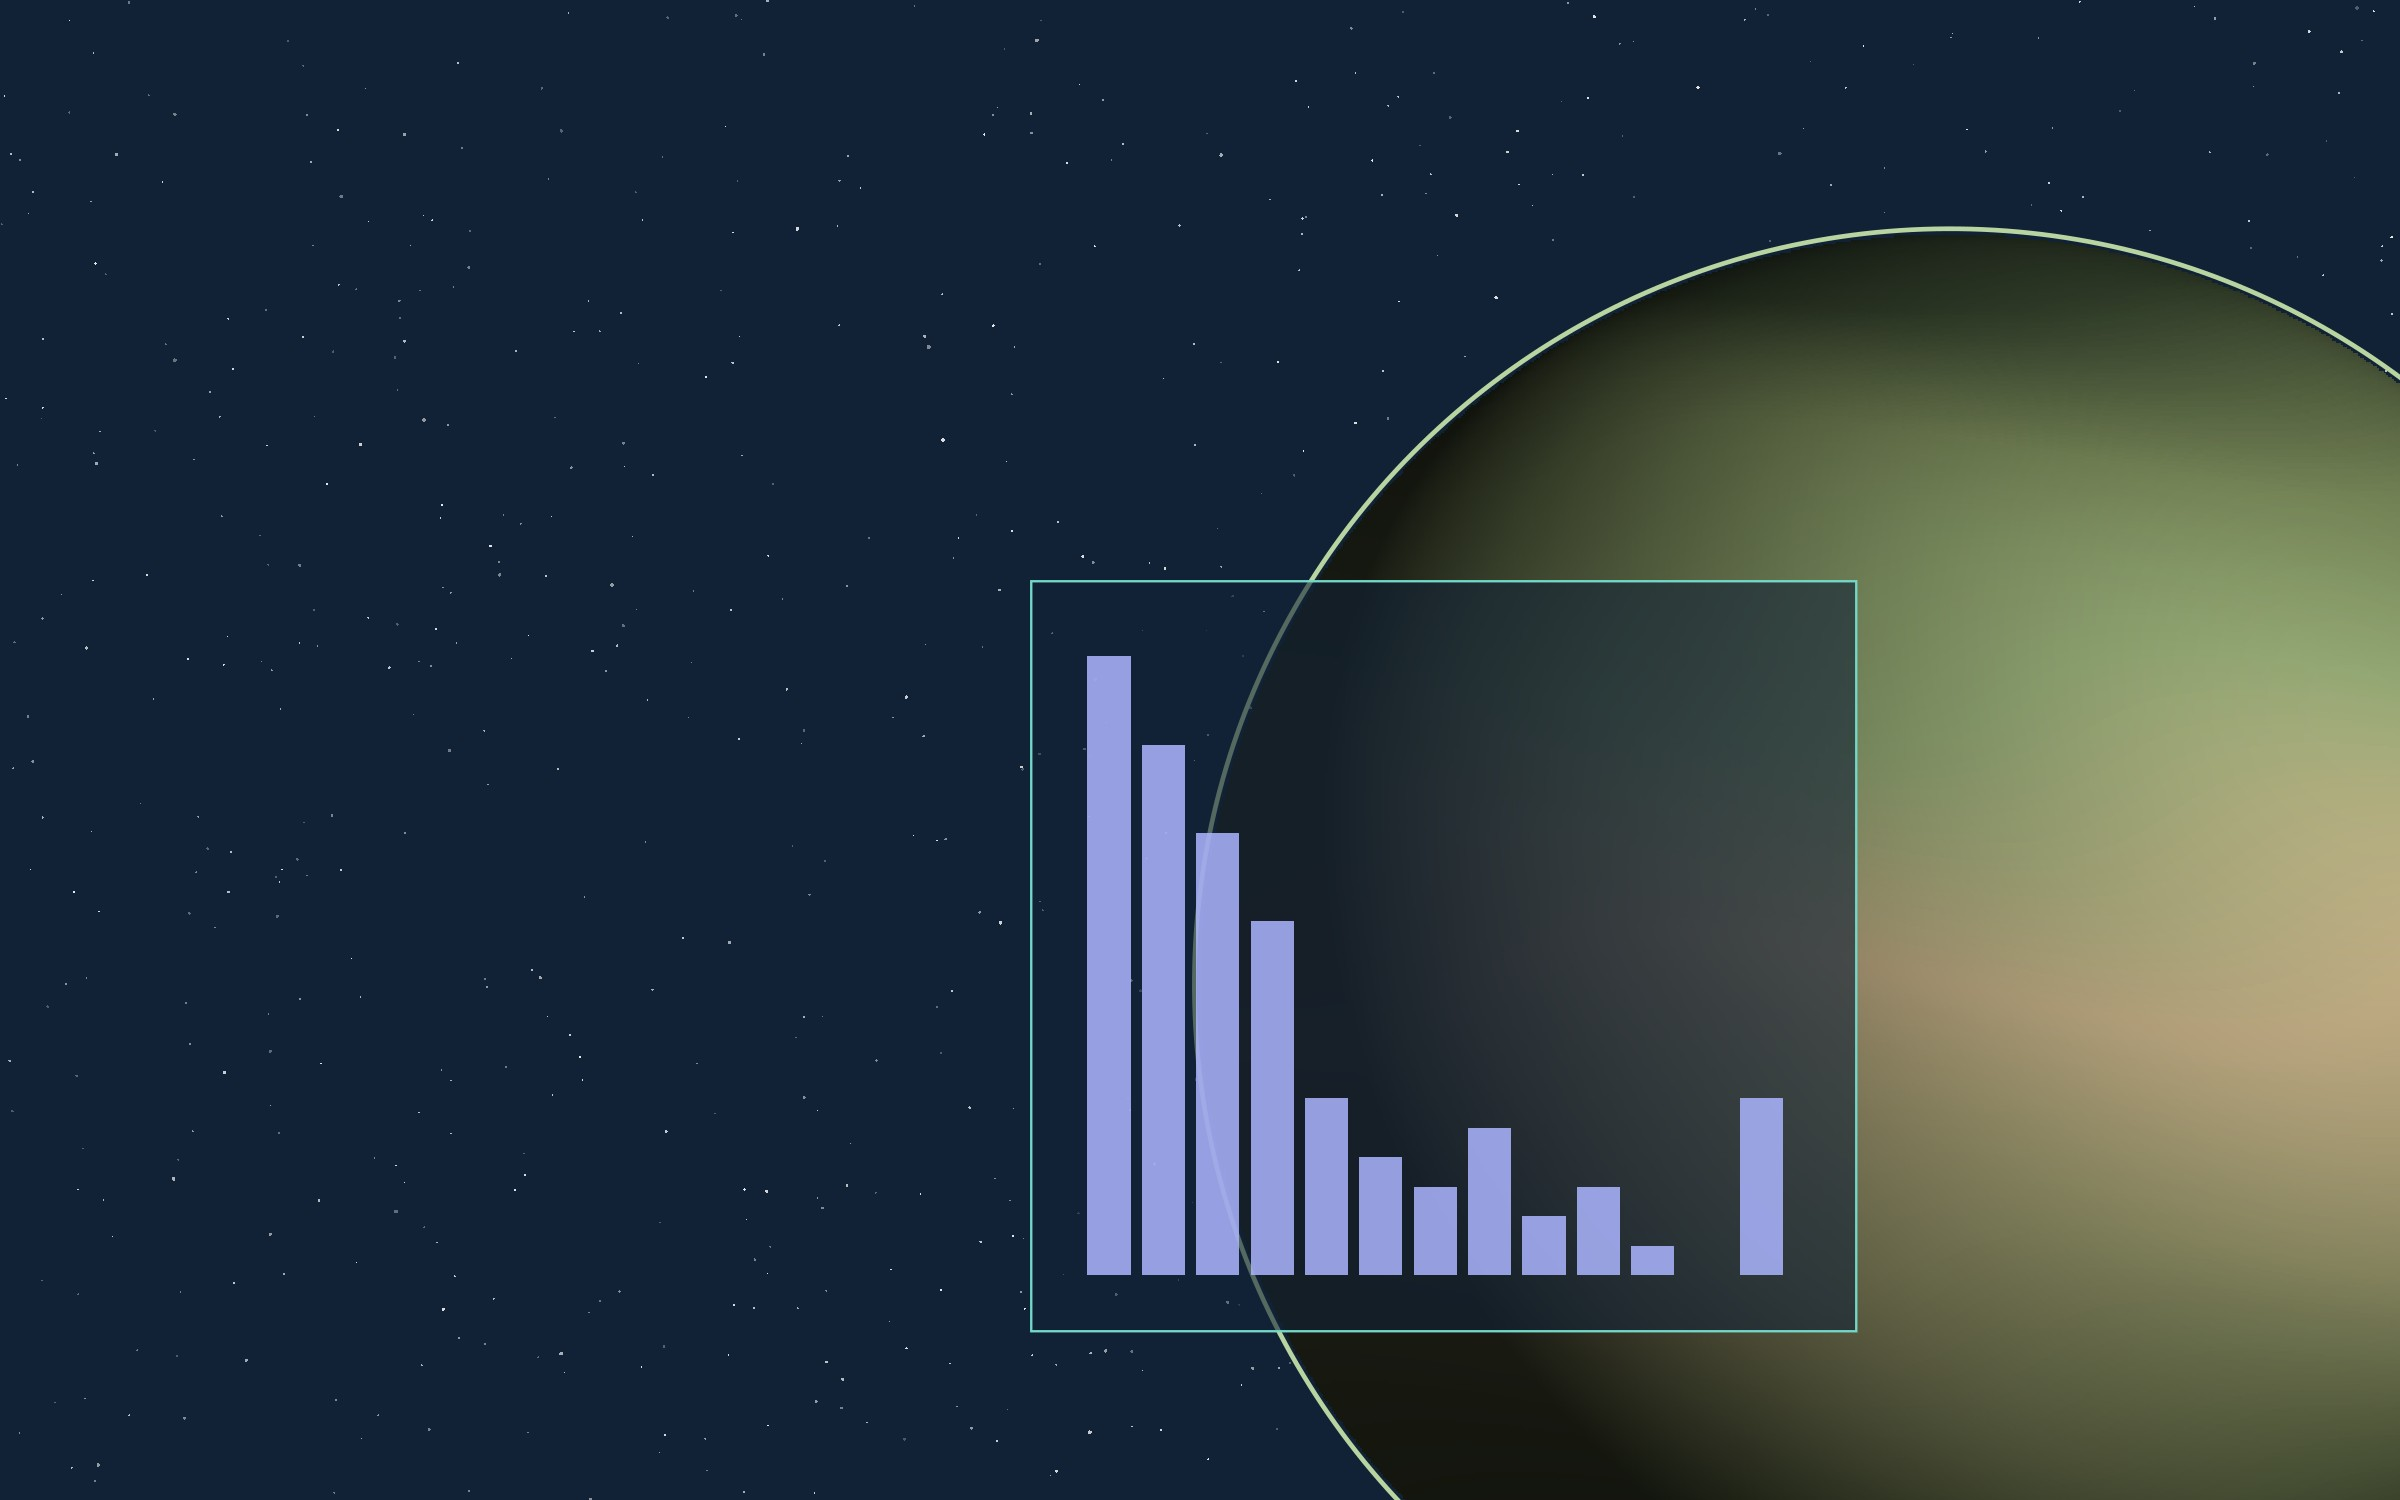
\includegraphics[width=20cm,height=12.5cm]{Scena/copertina.jpg}};}{}
\node[anchor=north west,inner sep=0] at([xshift=1.05cm,yshift=-1.10cm]current page.north west){\color{Mint}\bfseries\fontsize{23}{28}\selectfont NUMERUS};
\node[anchor=north west,inner sep=0] at([xshift=1.07cm,yshift=-2.16cm]current page.north west){\color{white}\fontsize{9}{12}\selectfont MODULO M20 · SCIENZE DELLA TERRA};
\draw[Mint,line width=1.5pt]([xshift=1.07cm,yshift=-2.78cm]current page.north west)--([xshift=2.6cm,yshift=-2.78cm]current page.north west);
\node[anchor=north west,inner sep=0] at([xshift=1.05cm,yshift=-3.35cm]current page.north west){\begin{minipage}{9.2cm}\raggedright\color{white}\bfseries\fontsize{28.5}{34.5}\selectfont Modelli lineari\\generalizzati\end{minipage}};
\node[anchor=north west,inner sep=0] at([xshift=1.07cm,yshift=-7.88cm]current page.north west){\begin{minipage}{8.9cm}\raggedright\color{Lilac}\fontsize{12.2}{17}\selectfont Conteggi e proporzioni\end{minipage}};
\node[anchor=north west,inner sep=0] at([xshift=1.07cm,yshift=-8.70cm]current page.north west){\begin{minipage}{8.9cm}\raggedright\color{white!75}\fontsize{10.3}{14.5}\selectfont Poisson, offset, sovradispersione e regressione logistica\end{minipage}};
\node[anchor=north west,inner sep=0] at([xshift=1.07cm,yshift=-10.52cm]current page.north west){\color{white}\fontsize{10.5}{14}\selectfont GeoStat Lab · corso di Marzio De Corato};
\node[anchor=north west,inner sep=0] at([xshift=1.07cm,yshift=-11.17cm]current page.north west){\color{Mint}\fontsize{8.8}{11}\selectfont\href{https://creativecommons.org/licenses/by-nc-sa/4.0/}{Impaginazione da Tessera · CC BY-NC-SA 4.0}};
\end{tikzpicture}\end{frame}

\begin{frame}[plain]\hypertarget{slide2}{}
\bookmark[level=1,page=2]{Indice della presentazione}
\begin{tikzpicture}[remember picture,overlay]
\PilotChrome{Indice della presentazione}{PERCORSO}{2}{I titoli dell’indice aprono i capitoli. Il nome del capitolo in alto riporta a questa pagina.}
\node[anchor=north west,inner sep=0] at([xshift=.96cm,yshift=-2.12cm]current page.north west){\Colonna{9.40cm}{\PLabel{Capitoli}
{\fontsize{10.7}{13.5}\selectfont\hyperlink{slide4}{Conteggi e regressione lineare\hfill 4}\par}\vspace{.16cm}
{\fontsize{10.7}{13.5}\selectfont\hyperlink{slide10}{Il modello di Poisson\hfill 10}\par}\vspace{.16cm}
{\fontsize{10.7}{13.5}\selectfont\hyperlink{slide17}{Sovradispersione\hfill 17}\par}\vspace{.16cm}
{\fontsize{10.7}{13.5}\selectfont\hyperlink{slide24}{Proporzioni e regressione logistica\hfill 24}\par}\vspace{.16cm}
}};
\node[anchor=north west,inner sep=0] at([xshift=10.85cm,yshift=-2.12cm]current page.north west){\Colonna{8.16cm}{\PLabel{Percorso di lettura}
\PBody{Novantasei celle di un bacino riportano il numero di frane, la superficie, la pendenza e la litologia; trentasei sezioni sottili riportano un conteggio per punti del feldspato lungo un percorso di trasporto. Il percorso va dai limiti della retta per i conteggi al modello di Poisson, alla sovradispersione e alle proporzioni.}
\PInfo{Le pagine Scenario A e Confronto riprendono gli esperimenti nel browser. I valori di partenza del simulatore possono differire dal caso guida.}
\href{https://marzione00.github.io/Lab_Geo/\#modulo-M20}{\color{Classical}\bfseries Apri gli esperimenti di Numerus}}};
\end{tikzpicture}\end{frame}

\begin{frame}[plain]\hypertarget{slide3}{}
\bookmark[level=1,page=3]{Quanto aumenta il tasso di frane con la pendenza?}
\begin{tikzpicture}[remember picture,overlay]
\PilotChrome{Quanto aumenta il tasso di frane con la pendenza?}{IL CASO GUIDA}{3}{Un conteggio è un intero non negativo: la sua varianza dipende dalla media.}
\node[anchor=north west,inner sep=0] at([xshift=.96cm,yshift=-2.12cm]current page.north west){\Colonna{9.40cm}{{\centering\resizebox{.97\linewidth}{!}{\begin{tikzpicture}[x=1cm,y=1cm,every node/.append style={anchor=center,inner sep=.3333em}]
\foreach \x/\n/\t/\col in {0.9/1/Conteggi/GeoA,3.0/2/Poisson/GeoC,5.1/3/{Sovra-\\dispersione}/GeoA,7.2/4/Proporzioni/GeoB}{
 \draw[\col,fill=\col!8,rounded corners=4pt,line width=.8pt] (\x-.95,1.25) rectangle(\x+.95,3.35);
 \node[font=\bfseries\fontsize{15}{18}\selectfont,text=\col] at(\x,2.75){\n};
 \node[pNote,text width=1.75cm,align=center] at(\x,1.85){\t};}
\foreach \x in {1.85,3.95,6.05}{\draw[pEdge] (\x,2.3)--(\x+.2,2.3);}
\draw[Rule,line width=.6pt] (0,.75)--(8.15,.75);
\node[pNote] at(4.08,.35){Interi non negativi e frazioni: una distribuzione e un legame per ciascuno.};
\end{tikzpicture}
}\par}
}};
\node[anchor=north west,inner sep=0] at([xshift=10.85cm,yshift=-2.12cm]current page.north west){\Colonna{8.16cm}{\PLabel{Il caso}
\PBody{Novantasei celle sintetiche di un bacino, con superfici fra 0,44 e 4 km$^2$, contengono in tutto 321 frane cartografate; ventuno celle non ne hanno nessuna. Per ogni cella sono note la pendenza media e la litologia prevalente: argille, flysch o calcari. Un secondo file riporta i punti di feldspato contati in 36 sezioni sottili.}
\PInfo{Seguiremo i dati dalla retta dei minimi quadrati al modello di Poisson con offset, alla sovradispersione con quasi-Poisson e binomiale negativa, fino alla regressione logistica per le proporzioni.}
}};
\end{tikzpicture}\end{frame}

\begin{frame}[plain]\hypertarget{slide4}{}
\bookmark[level=0,page=4]{Conteggi e regressione lineare}
\bookmark[level=1,page=4]{Che cosa prevede una retta per i conteggi?}
\begin{tikzpicture}[remember picture,overlay]
\PilotChrome{Che cosa prevede una retta per i conteggi?}{CONTEGGI E REGRESSIONE LINEARE}{4}{Una retta non conosce i vincoli di un conteggio: può prevedere valori negativi.}
\node[anchor=north west,inner sep=0] at([xshift=.96cm,yshift=-2.12cm]current page.north west){\Colonna{9.40cm}{\PLabel{Domanda}
\PBody{Il numero di frane per cella ha media 3,34. Che varianza hanno i conteggi? Che cosa prevede la retta dei minimi quadrati per una cella con pendenza di 4 gradi?}
\vspace{.35cm}\PLabel{Interpretazione}
\PBody{La varianza vale 15,07, quattro volte e mezzo la media, e ventuno celle hanno zero frane. La retta prevede $-0{,}60$ frane per una cella con pendenza di 4 gradi: un valore impossibile.}
}};
\node[anchor=north west,inner sep=0] at([xshift=10.85cm,yshift=-2.12cm]current page.north west){\Colonna{8.16cm}{\begin{tcolorbox}[enhanced,arc=1.7mm,boxrule=.6pt,colback=white,colframe=Classical!60!Navy,colbacktitle=Navy,coltitle=white,fonttitle=\bfseries\small,title={R · calcolo riproducibile},left=1.7mm,right=1.3mm,top=1.1mm,bottom=1.1mm,before skip=1mm,after skip=1.0mm]\lstinputlisting[style=GeoR,language=R]{Codice/capitolo-01.R}\end{tcolorbox}
\PLabel{Risultato in R}
\begin{tcolorbox}[colback=GeoTint,colframe=Rule,boxrule=.5pt,arc=1.4mm,left=2mm,right=1mm,top=1mm,bottom=1mm]{\fontsize{8.6}{11.4}\selectfont\ttfamily \mbox{\ \ \ media\ varianza\ \ \ \ \ zeri}\\\mbox{\ \ \ \ 3.34\ \ \ \ 15.07\ \ \ \ 21.00}\\\mbox{\ \ \ \ \ \ \ \ \ 1}\\\mbox{-0.6010453}}\end{tcolorbox}}};
\end{tikzpicture}\end{frame}

\begin{frame}[plain]\hypertarget{slide5}{}
\bookmark[level=1,page=5]{Frane, pendenza e litologia}
\begin{tikzpicture}[remember picture,overlay]
\PilotChrome{Frane, pendenza e litologia}{CONTEGGI E REGRESSIONE LINEARE}{5}{La densità di frane cresce con la pendenza in modo moltiplicativo, e il livello dipende dalla litologia.}
\node[anchor=north west,inner sep=0] at([xshift=.96cm,yshift=-2.12cm]current page.north west){\Colonna{9.40cm}{{\centering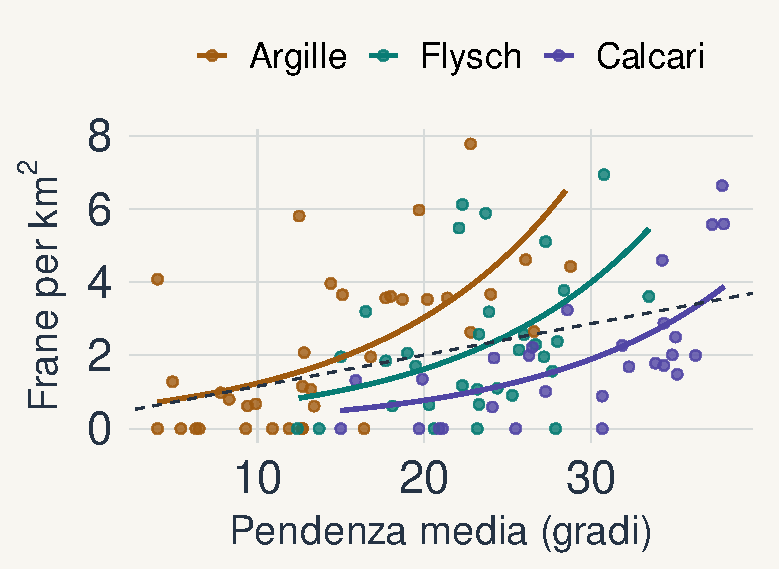
\includegraphics[width=\linewidth,height=6.15cm,keepaspectratio]{Figure/F01.pdf}\par}
\PSmall{Frane per km$^2$ e pendenza; curve: modello di Poisson per litologia nell’intervallo osservato; tratteggio: retta dei minimi quadrati.}
}};
\node[anchor=north west,inner sep=0] at([xshift=10.85cm,yshift=-2.12cm]current page.north west){\Colonna{8.16cm}{\PBody{Il bacino conta 2,36 frane per km$^2$ di superficie totale. Le curve del modello di Poisson crescono in modo esponenziale e restano positive; la retta tratteggiata attraversa lo zero a bassa pendenza. A parità di pendenza le argille hanno le densità maggiori e i calcari le minori.}
\PSmall{La densità è il conteggio diviso per la superficie della cella.}
}};
\end{tikzpicture}\end{frame}

\begin{frame}[plain]\hypertarget{slide6}{}
\bookmark[level=1,page=6]{Le tre parti di un modello lineare generalizzato}
\begin{tikzpicture}[remember picture,overlay]
\PilotChrome{Le tre parti di un modello lineare generalizzato}{CONTEGGI E REGRESSIONE LINEARE}{6}{Distribuzione, predittore lineare e funzione di legame si scelgono separatamente.}
\node[anchor=north west,inner sep=0] at([xshift=.96cm,yshift=-2.12cm]current page.north west){\Colonna{9.40cm}{{\centering\resizebox{0.94\linewidth}{!}{\begin{tikzpicture}[x=1cm,y=1cm,every node/.append style={anchor=center,inner sep=.3333em}]
\node[pFlow,text width=2.6cm] (a) at(0,2.6){\textbf{Componente casuale}\\$Y_i\sim$ Poisson$(\mu_i)$};
\node[pFlow,text width=2.6cm] (b) at(6,2.6){\textbf{Predittore lineare}\\$\eta_i=\beta_0+\beta_1x_i$};
\node[pFlow,text width=2.6cm] (c) at(3,0){\textbf{Funzione di legame}\\$\log\mu_i=\eta_i$};
\draw[pEdge] (b)--(c);
\draw[pEdge] (c)--(a);
\node[pNote,text width=7.4cm] at(3,-1.75){Il legame collega la media alla scala del predittore: con il logaritmo ogni $\mu_i$ resta positivo e gli effetti dei predittori si moltiplicano. L’offset aggiunge $\log A_i$ a $\eta_i$ con coefficiente 1.};
\end{tikzpicture}
}\par}
\PSmall{Componente casuale, predittore lineare e funzione di legame.}
}};
\node[anchor=north west,inner sep=0] at([xshift=10.85cm,yshift=-2.12cm]current page.north west){\Colonna{8.16cm}{\PBody{John Nelder e Robert Wedderburn riunirono nel 1972 modelli per dati normali, binomiali, di Poisson e gamma in un’unica classe. La distribuzione descrive la variabilità di ogni osservazione, il predittore lineare combina i predittori, il legame collega la media al predittore. Per i conteggi il legame logaritmico mantiene positiva la media.}
\par\smallskip{\centering\adjustbox{max width=.98\linewidth}{$\displaystyle \log\mu_i=\log A_i+\mathbf x_i^{\mathsf T}\boldsymbol\beta$}\par\smallskip}
\PSmall{$Y_i\sim\mathrm{Poisson}(\mu_i)$; $A_i$ è la superficie della cella e $\log A_i$ l’offset.}
}};
\end{tikzpicture}\end{frame}

\begin{frame}[plain]\hypertarget{slide7}{}
\bookmark[level=1,page=7]{Il modello di Poisson con offset}
\begin{tikzpicture}[remember picture,overlay]
\PilotChrome{Il modello di Poisson con offset}{CONTEGGI E REGRESSIONE LINEARE}{7}{L’offset $\log A_i$ trasforma il modello dei conteggi in un modello dei tassi per unità di superficie.}
\node[anchor=north west,inner sep=0] at([xshift=.96cm,yshift=-2.12cm]current page.north west){\Colonna{9.40cm}{\PBody{Il codice adatta il modello con \texttt{glm}, famiglia di Poisson e offset \texttt{log(area\_km2)}. Il coefficiente della pendenza vale 0,0895 per grado: ogni 10 gradi il tasso di frane per km$^2$ si moltiplica per $e^{0{,}895}=2{,}45$. I coefficienti delle litologie sono negativi rispetto alle argille.}
\par\smallskip{\centering\adjustbox{max width=.98\linewidth}{$\displaystyle \frac{\mu(x+10)}{\mu(x)}=e^{10\beta_1}$}\par\smallskip}
}};
\node[anchor=north west,inner sep=0] at([xshift=10.85cm,yshift=-2.12cm]current page.north west){\Colonna{8.16cm}{\begin{tcolorbox}[enhanced,arc=1.7mm,boxrule=.6pt,colback=white,colframe=Classical!60!Navy,colbacktitle=Navy,coltitle=white,fonttitle=\bfseries\small,title={R · calcolo riproducibile},left=1.7mm,right=1.3mm,top=1.1mm,bottom=1.1mm,before skip=1mm,after skip=1.0mm]\lstinputlisting[style=GeoR,language=R]{Codice/capitolo-02.R}\end{tcolorbox}
\PLabel{Risultato in R}
\begin{tcolorbox}[colback=GeoTint,colframe=Rule,boxrule=.5pt,arc=1.4mm,left=2mm,right=1mm,top=1mm,bottom=1mm]{\fontsize{8.6}{11.4}\selectfont\ttfamily \mbox{\ \ \ \ \ \ \ \ \ \ \ \ \ \ \ \ \ \ \ stima}\\\mbox{(Intercept)\ \ \ \ \ \ -0.6807}\\\mbox{pendenza\ \ \ \ \ \ \ \ \ \ 0.0895}\\\mbox{litologiaCalcari\ -1.3673}\\\mbox{litologiaFlysch\ \ -0.6228}\\\mbox{[1]\ 2.449}}\end{tcolorbox}}};
\end{tikzpicture}\end{frame}

\begin{frame}[plain]\hypertarget{slide8}{}
\bookmark[level=1,page=8]{Retta e modello di Poisson per i conteggi}
\begin{tikzpicture}[remember picture,overlay]
\PilotChrome{Retta e modello di Poisson per i conteggi}{CONTEGGI E REGRESSIONE LINEARE}{8}{Confrontare retta e modello di Poisson su conteggi che crescono in modo esponenziale.}
\node[anchor=north west,inner sep=0] at([xshift=.96cm,yshift=-2.12cm]current page.north west){\Colonna{9.40cm}{{\centering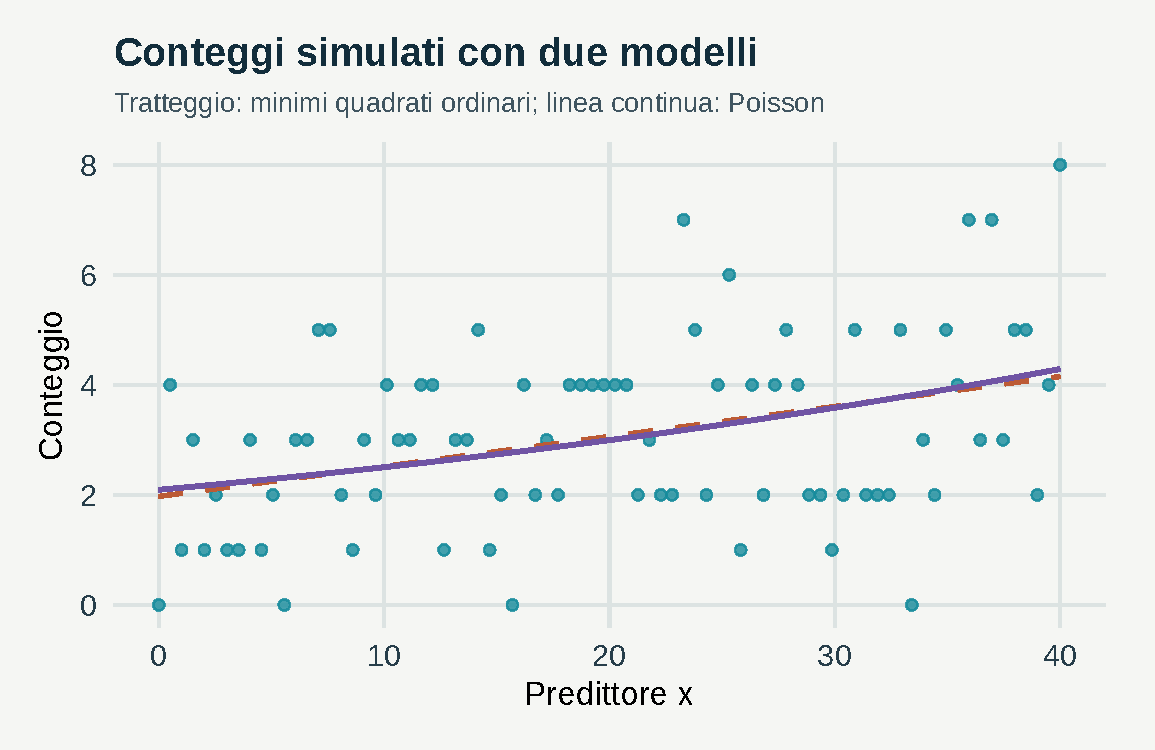
\includegraphics[width=\linewidth,height=6.0cm,keepaspectratio]{Esperimenti/m20-lineare-A.pdf}\par}
\PSmall{Pendenza del logaritmo della media: 0,03. Seme: 17.}
}};
\node[anchor=north west,inner sep=0] at([xshift=10.85cm,yshift=-2.12cm]current page.north west){\Colonna{8.16cm}{\PLabel{Scenario A · simulazione}
\PBody{L’esperimento genera ottanta conteggi di Poisson con media $3e^{b(x-20)}$ e adatta una retta e un modello di Poisson. Con $b=0{,}03$ la retta non prevede valori negativi, e la varianza dei residui passa da 1,83 a 3,34 fra le due metà dell’intervallo.}
\par\smallskip{\centering\adjustbox{max width=.98\linewidth}{$\displaystyle \log\mu_i=\beta_0+\beta_1x_i,\qquad \operatorname{var}(Y_i)=\mu_i$}\par\smallskip}
\PSmall{Il rapporto di tasso stimato, 1,20, e quello vero, 1,35, differiscono per la variabilità campionaria.}
}};
\node[anchor=north east,inner sep=0] at([xshift=17.1cm,yshift=-12.04cm]current page.north west){\fontsize{7.7}{9}\selectfont \href{https://marzione00.github.io/Lab_Geo/\#laboratorio/m20-lineare}{\color{Classical}\bfseries Apri il laboratorio · m20-lineare}};
\end{tikzpicture}\end{frame}

\begin{frame}[plain]\hypertarget{slide9}{}
\bookmark[level=1,page=9]{Confronto | Retta e modello di Poisson}
\begin{tikzpicture}[remember picture,overlay]
\PilotChrome{Confronto | Retta e modello di Poisson}{CONTEGGI E REGRESSIONE LINEARE}{9}{Con una crescita forte la retta prevede conteggi negativi e ignora la varianza crescente.}
\node[anchor=north west,inner sep=0] at([xshift=.96cm,yshift=-2.12cm]current page.north west){\Colonna{9.40cm}{{\centering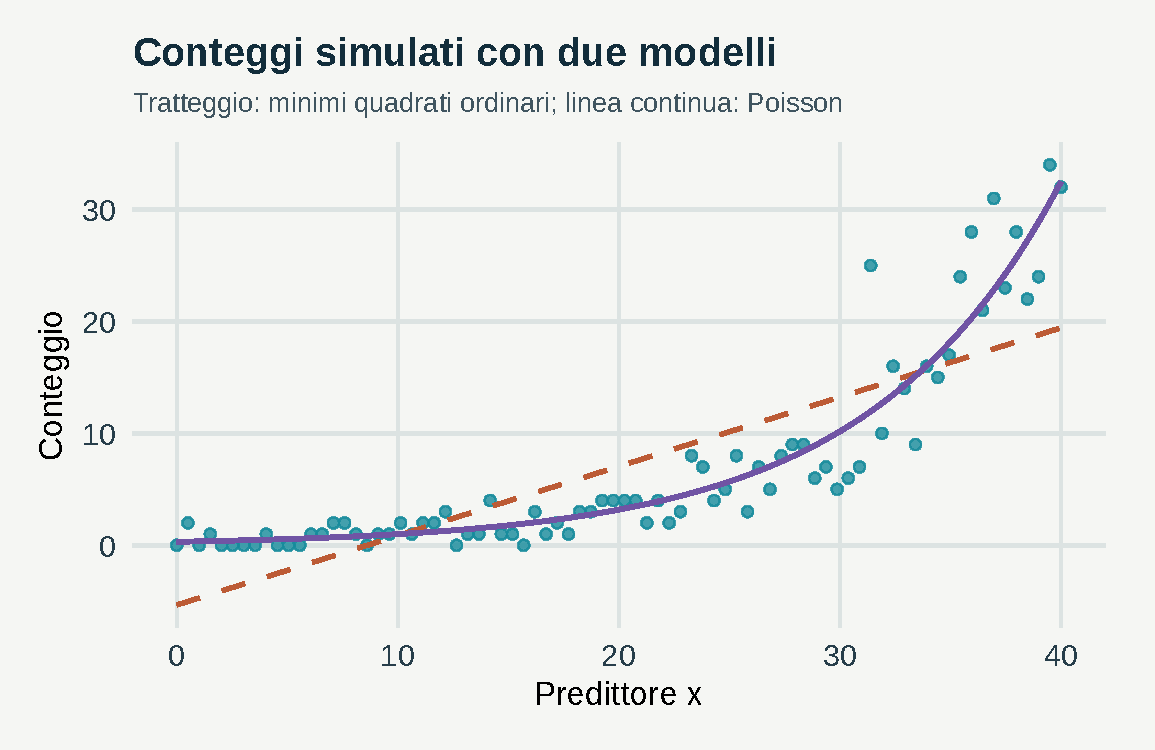
\includegraphics[width=\linewidth,height=5.6cm,keepaspectratio]{Esperimenti/m20-lineare-B.pdf}\par}
\PSmall{Pendenza del logaritmo della media: 0,03 $\to$ 0,12. Il seme è fisso.}
}};
\node[anchor=north west,inner sep=0] at([xshift=10.85cm,yshift=-2.12cm]current page.north west){\Colonna{8.16cm}{\PLabel{Confronto fra gli scenari}
{\fontsize{10.2}{12.8}\selectfont\begin{tabular}{@{}>{\raggedright\arraybackslash}p{0.48\linewidth}@{\hspace{.13cm}}>{\raggedright\arraybackslash}p{0.224\linewidth}@{\hspace{.13cm}}>{\raggedright\arraybackslash}p{0.224\linewidth}@{}}\toprule Grandezza & A & B\\[2.3pt]
\midrule 
Previsioni negative & 0 & 0{,}215\\[2.3pt]
Varianza dei residui, $x<20$ & 1{,}83 & 9{,}45\\[2.3pt]
Varianza dei residui, $x\ge20$ & 3{,}34 & 43{,}5\\[2.3pt]
Rapporto di tasso, Poisson & 1{,}2 & 3{,}19\\[2.3pt]
Rapporto di tasso vero & 1{,}35 & 3{,}32\\[2.3pt]
\bottomrule\end{tabular}\par}
\vspace{.25cm}\PBody{Con $b=0{,}12$ la retta prevede valori negativi nel 21,5\% dell’intervallo e la varianza dei residui passa da 9,45 a 43,5; il modello di Poisson stima 3,19 contro 3,32.}
}};
\node[anchor=north east,inner sep=0] at([xshift=17.1cm,yshift=-12.04cm]current page.north west){\fontsize{7.7}{9}\selectfont \href{https://marzione00.github.io/Lab_Geo/\#laboratorio/m20-lineare}{\color{Classical}\bfseries Apri il laboratorio · m20-lineare}};
\end{tikzpicture}\end{frame}

\begin{frame}[plain]\hypertarget{slide10}{}
\bookmark[level=0,page=10]{Il modello di Poisson}
\bookmark[level=1,page=10]{Minimi quadrati pesati ripetuti}
\begin{tikzpicture}[remember picture,overlay]
\PilotChrome{Minimi quadrati pesati ripetuti}{IL MODELLO DI POISSON}{10}{Un modello lineare generalizzato si adatta con una sequenza di regressioni pesate.}
\node[anchor=north west,inner sep=0] at([xshift=.96cm,yshift=-2.12cm]current page.north west){\Colonna{9.40cm}{{\centering\resizebox{0.94\linewidth}{!}{\begin{tikzpicture}[x=1cm,y=1cm,every node/.append style={anchor=center,inner sep=.3333em}]
\node[pFlow,text width=2.9cm] (a) at(0,2.4){\textbf{1. Media corrente}\\$\mu_i=e^{\eta_i}$};
\node[pFlow,text width=2.9cm] (b) at(5.6,2.4){\textbf{2. Variabile di lavoro}\\$z_i=\eta_i+\dfrac{y_i-\mu_i}{\mu_i}$};
\node[pFlow,text width=2.9cm] (c) at(5.6,0){\textbf{3. Pesi}\\$w_i=\mu_i$};
\node[pFlow,text width=2.9cm] (d) at(0,0){\textbf{4. Minimi quadrati pesati}\\di $z$ su $x$};
\draw[pEdge] (a)--(b);\draw[pEdge] (b)--(c);\draw[pEdge] (c)--(d);\draw[pEdge] (d)--(a);
\node[pNote,text width=7.6cm] at(2.8,-1.65){Si ripete fino alla convergenza: le stime coincidono con quelle di massima verosimiglianza (Nelder e Wedderburn, 1972).};
\end{tikzpicture}
}\par}
\PSmall{Le quattro fasi dell’algoritmo per il modello di Poisson con legame logaritmico.}
}};
\node[anchor=north west,inner sep=0] at([xshift=10.85cm,yshift=-2.12cm]current page.north west){\Colonna{8.16cm}{\PBody{Nelder e Wedderburn mostrarono che le stime di massima verosimiglianza si ottengono ripetendo una regressione lineare pesata su una variabile di lavoro. \texttt{M20\_figure.R} implementa l’algoritmo in poche righe e ottiene gli stessi coefficienti di \texttt{glm} entro $10^{-8}$.}
\par\smallskip{\centering\adjustbox{max width=.98\linewidth}{$\displaystyle \boldsymbol\beta\leftarrow(X^{\mathsf T}WX)^{-1}X^{\mathsf T}W\mathbf z$}\par\smallskip}
}};
\end{tikzpicture}\end{frame}

\begin{frame}[plain]\hypertarget{slide11}{}
\bookmark[level=1,page=11]{Rapporti fra tassi}
\begin{tikzpicture}[remember picture,overlay]
\PilotChrome{Rapporti fra tassi}{IL MODELLO DI POISSON}{11}{Su scala logaritmica un rapporto di tasso pari a 1 indica nessun effetto.}
\node[anchor=north west,inner sep=0] at([xshift=.96cm,yshift=-2.12cm]current page.north west){\Colonna{9.40cm}{{\centering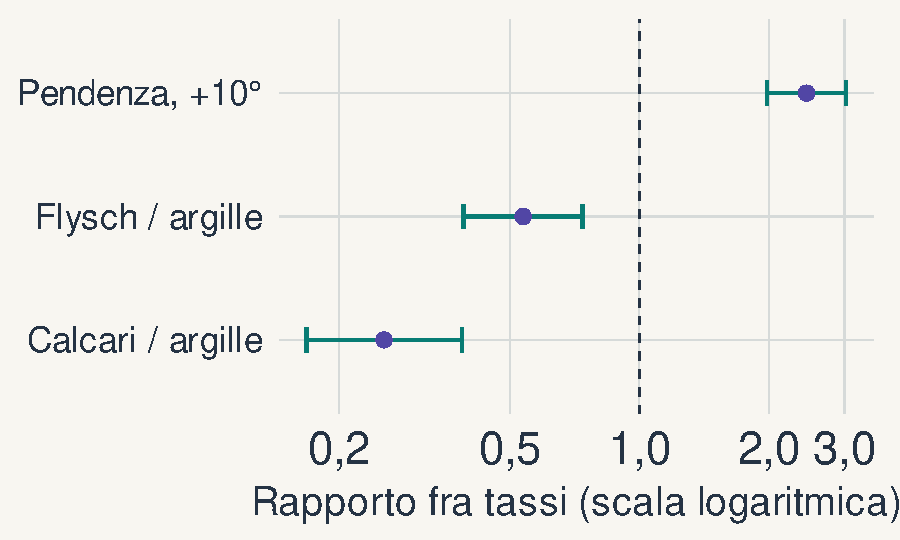
\includegraphics[width=\linewidth,height=6.15cm,keepaspectratio]{Figure/F02.pdf}\par}
\PSmall{Rapporti fra tassi del modello di Poisson con intervalli di Wald al 95\%; asse logaritmico.}
}};
\node[anchor=north west,inner sep=0] at([xshift=10.85cm,yshift=-2.12cm]current page.north west){\Colonna{8.16cm}{\PBody{Dieci gradi di pendenza in più moltiplicano il tasso per 2,45, con intervallo da 1,98 a 3,03. A parità di pendenza il flysch ha un tasso pari a 0,54 volte quello delle argille, i calcari 0,25 volte. Gli intervalli presuppongono che i conteggi seguano una distribuzione di Poisson.}
\PSmall{L’intervallo di Wald è $e^{\hat\beta\pm1{,}96\,\mathrm{se}}$, asimmetrico sulla scala dei rapporti.}
}};
\end{tikzpicture}\end{frame}

\begin{frame}[plain]\hypertarget{slide12}{}
\bookmark[level=1,page=12]{Come si leggono i coefficienti?}
\begin{tikzpicture}[remember picture,overlay]
\PilotChrome{Come si leggono i coefficienti?}{IL MODELLO DI POISSON}{12}{L’esponenziale di un coefficiente è un rapporto fra tassi, a parità degli altri predittori.}
\node[anchor=north west,inner sep=0] at([xshift=.96cm,yshift=-2.12cm]current page.north west){\Colonna{9.40cm}{\PLabel{Domanda}
\PBody{Il coefficiente del flysch vale $-0{,}623$. Che cosa significa per il tasso di frane di una cella di flysch rispetto a una cella di argille con la stessa pendenza?}
\vspace{.35cm}\PLabel{Interpretazione}
\PBody{Il tasso vale $e^{-0{,}623}=0{,}536$ volte quello delle argille, con intervallo da 0,390 a 0,739: circa la metà. Un grado di pendenza in più moltiplica il tasso per 1,094.}
}};
\node[anchor=north west,inner sep=0] at([xshift=10.85cm,yshift=-2.12cm]current page.north west){\Colonna{8.16cm}{\begin{tcolorbox}[enhanced,arc=1.7mm,boxrule=.6pt,colback=white,colframe=Classical!60!Navy,colbacktitle=Navy,coltitle=white,fonttitle=\bfseries\small,title={R · calcolo riproducibile},left=1.7mm,right=1.3mm,top=1.1mm,bottom=1.1mm,before skip=1mm,after skip=1.0mm]\lstinputlisting[style=GeoR,language=R]{Codice/capitolo-03.R}\end{tcolorbox}
\PLabel{Risultato in R}
\begin{tcolorbox}[colback=GeoTint,colframe=Rule,boxrule=.5pt,arc=1.4mm,left=2mm,right=1mm,top=1mm,bottom=1mm]{\fontsize{8.6}{11.4}\selectfont\ttfamily \mbox{\ \ \ \ \ \ \ \ \ \ \ \ \ \ \ \ \ stima\ \ \ inf\ \ \ sup}\\\mbox{pendenza\ \ \ \ \ \ \ \ \ 1.094\ 1.071\ 1.117}\\\mbox{litologiaFlysch\ \ 0.536\ 0.390\ 0.739}\\\mbox{litologiaCalcari\ 0.255\ 0.168\ 0.387}}\end{tcolorbox}}};
\end{tikzpicture}\end{frame}

\begin{frame}[plain]\hypertarget{slide13}{}
\bookmark[level=1,page=13]{La devianza e il test del rapporto di verosimiglianza}
\begin{tikzpicture}[remember picture,overlay]
\PilotChrome{{\fontsize{15.3}{19}\selectfont La devianza e il test del rapporto di verosimiglianza}}{IL MODELLO DI POISSON}{13}{La differenza di devianza fra modelli annidati segue approssimativamente una chi quadrato.}
\node[anchor=north west,inner sep=0] at([xshift=.96cm,yshift=-2.12cm]current page.north west){\Colonna{9.40cm}{\PBody{La devianza misura la distanza fra il modello e un modello con un parametro per ogni osservazione. Togliendo la litologia la devianza passa da 153,21 a 195,13: la differenza, 41,92 con due gradi di libertà, ha probabilità di coda $7{,}9\cdot10^{-10}$. La litologia migliora il modello.}
\par\smallskip{\centering\adjustbox{max width=.98\linewidth}{$\displaystyle D=2\sum_i\Big[y_i\log\frac{y_i}{\hat\mu_i}-(y_i-\hat\mu_i)\Big]$}\par\smallskip}
}};
\node[anchor=north west,inner sep=0] at([xshift=10.85cm,yshift=-2.12cm]current page.north west){\Colonna{8.16cm}{\begin{tcolorbox}[enhanced,arc=1.7mm,boxrule=.6pt,colback=white,colframe=Classical!60!Navy,colbacktitle=Navy,coltitle=white,fonttitle=\bfseries\small,title={R · calcolo riproducibile},left=1.7mm,right=1.3mm,top=1.1mm,bottom=1.1mm,before skip=1mm,after skip=1.0mm]\lstinputlisting[style=GeoR,language=R]{Codice/capitolo-04.R}\end{tcolorbox}
\PLabel{Risultato in R}
\begin{tcolorbox}[colback=GeoTint,colframe=Rule,boxrule=.5pt,arc=1.4mm,left=2mm,right=1mm,top=1mm,bottom=1mm]{\fontsize{8.6}{11.4}\selectfont\ttfamily \mbox{dev\_m0\ dev\_m1\ \ \ \ \ \ D}\\\mbox{195.13\ 153.21\ \ 41.92}\\\mbox{[1]\ 7.88e-10}}\end{tcolorbox}}};
\end{tikzpicture}\end{frame}

\begin{frame}[plain]\hypertarget{slide14}{}
\bookmark[level=1,page=14]{Frequenze osservate e attese}
\begin{tikzpicture}[remember picture,overlay]
\PilotChrome{Frequenze osservate e attese}{IL MODELLO DI POISSON}{14}{Troppi zeri e troppi valori grandi rispetto al modello segnalano sovradispersione.}
\node[anchor=north west,inner sep=0] at([xshift=.96cm,yshift=-2.12cm]current page.north west){\Colonna{9.40cm}{{\centering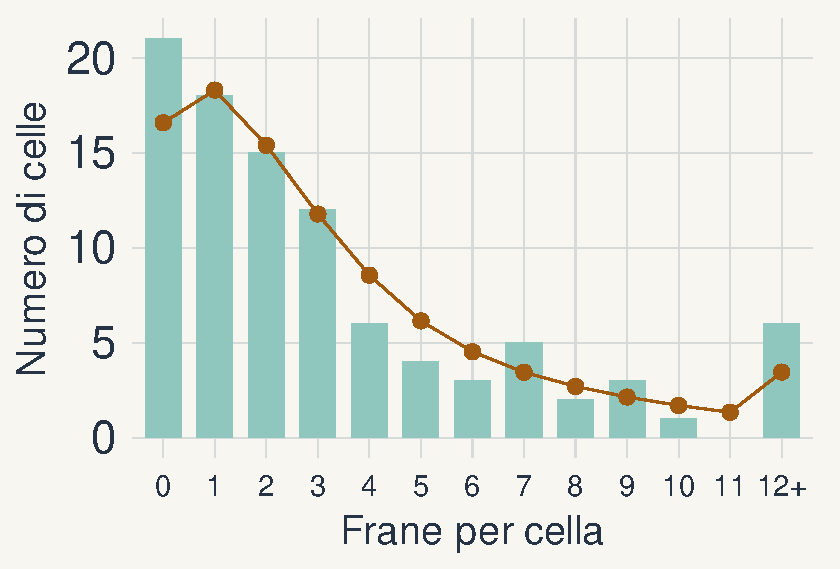
\includegraphics[width=\linewidth,height=6.15cm,keepaspectratio]{Figure/F03.pdf}\par}
\PSmall{Numero di celle per numero di frane: barre osservate, punti attesi dal modello di Poisson.}
}};
\node[anchor=north west,inner sep=0] at([xshift=10.85cm,yshift=-2.12cm]current page.north west){\Colonna{8.16cm}{\PBody{Il modello di Poisson attende 16,6 celle senza frane: ce ne sono 21. Le celle con 12 frane o più sono 6 contro 3,4 attese, e quelle con 4, 5 e 6 frane sono meno del previsto. I conteggi sono più dispersi di quanto il modello preveda. La devianza residua vale 153,2 con 92 gradi di libertà.}
\PSmall{Le frequenze attese sommano le probabilità di Poisson delle 96 celle.}
}};
\end{tikzpicture}\end{frame}

\begin{frame}[plain]\hypertarget{slide15}{}
\bookmark[level=1,page=15]{Offset e superfici diverse}
\begin{tikzpicture}[remember picture,overlay]
\PilotChrome{Offset e superfici diverse}{IL MODELLO DI POISSON}{15}{Valutare la stima del rapporto di tasso con e senza offset quando la superficie dipende dal predittore.}
\node[anchor=north west,inner sep=0] at([xshift=.96cm,yshift=-2.12cm]current page.north west){\Colonna{9.40cm}{{\centering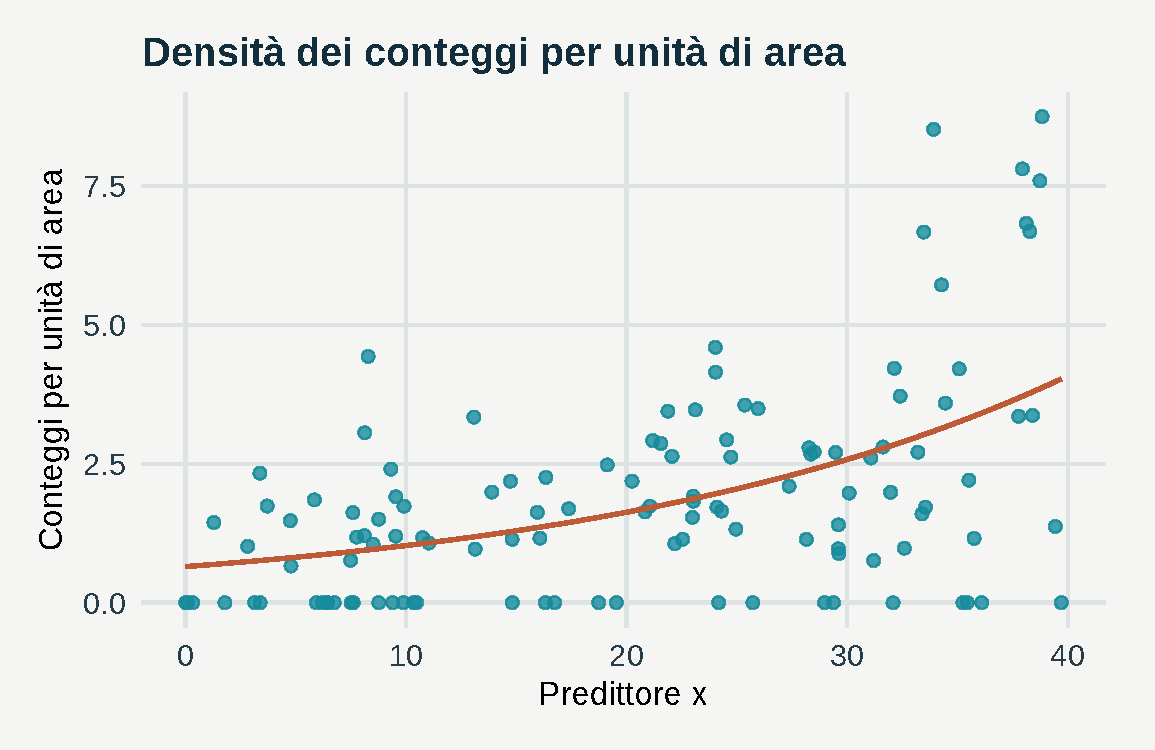
\includegraphics[width=\linewidth,height=6.0cm,keepaspectratio]{Esperimenti/m20-offset-A.pdf}\par}
\PSmall{Superficie indipendente dal predittore. Seme: 17.}
}};
\node[anchor=north west,inner sep=0] at([xshift=10.85cm,yshift=-2.12cm]current page.north west){\Colonna{8.16cm}{\PLabel{Scenario A · simulazione}
\PBody{L’esperimento genera centoventi celle con un tasso che cresce con $x$, rapporto vero 1,65 per 10 unità. Se la superficie non dipende da $x$, le stime con offset e senza valgono 1,63 e 1,56.}
\par\smallskip{\centering\adjustbox{max width=.98\linewidth}{$\displaystyle \log\mu_i=\log A_i+\beta_0+\beta_1x_i$}\par\smallskip}
\PSmall{Senza offset la superficie entra nell’errore del modello.}
}};
\node[anchor=north east,inner sep=0] at([xshift=17.1cm,yshift=-12.04cm]current page.north west){\fontsize{7.7}{9}\selectfont \href{https://marzione00.github.io/Lab_Geo/\#laboratorio/m20-offset}{\color{Classical}\bfseries Apri il laboratorio · m20-offset}};
\end{tikzpicture}\end{frame}

\begin{frame}[plain]\hypertarget{slide16}{}
\bookmark[level=1,page=16]{Confronto | Offset e superfici diverse}
\begin{tikzpicture}[remember picture,overlay]
\PilotChrome{Confronto | Offset e superfici diverse}{IL MODELLO DI POISSON}{16}{Senza offset il predittore assorbe l’effetto della superficie a cui è correlato.}
\node[anchor=north west,inner sep=0] at([xshift=.96cm,yshift=-2.12cm]current page.north west){\Colonna{9.40cm}{{\centering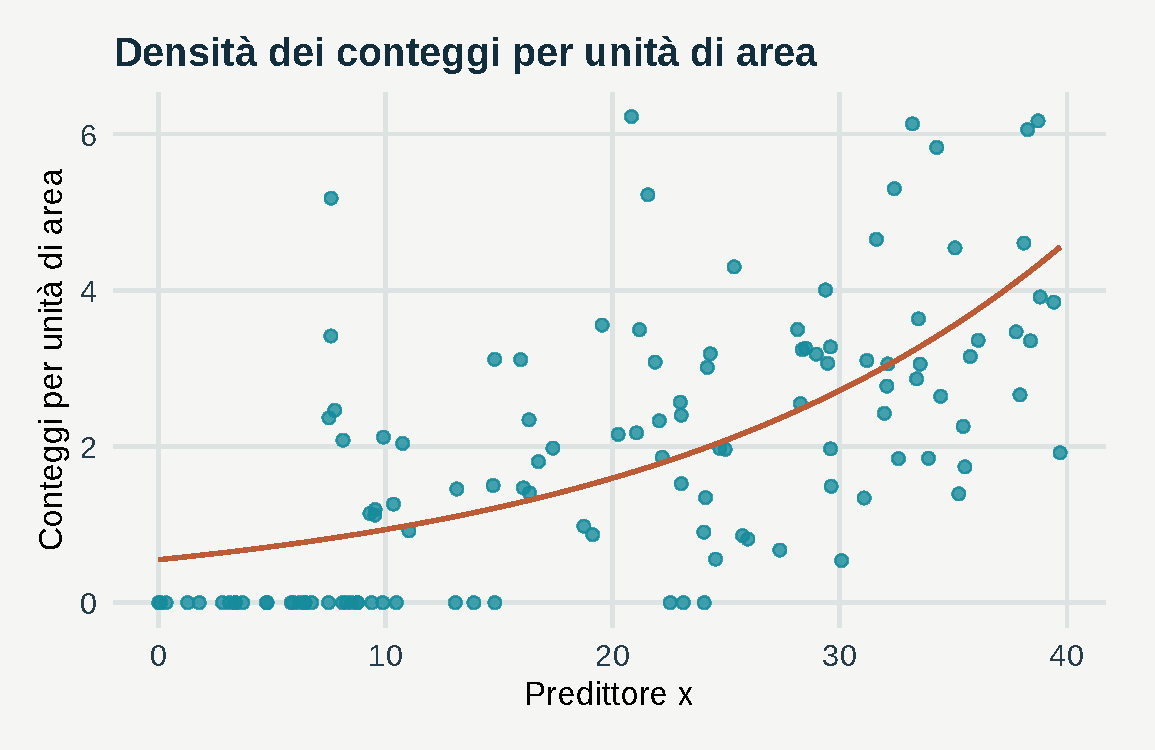
\includegraphics[width=\linewidth,height=5.6cm,keepaspectratio]{Esperimenti/m20-offset-B.pdf}\par}
\PSmall{Dipendenza di log(area) dal predittore: 0 $\to$ 0,6 per 10 unità. Il seme è fisso.}
}};
\node[anchor=north west,inner sep=0] at([xshift=10.85cm,yshift=-2.12cm]current page.north west){\Colonna{8.16cm}{\PLabel{Confronto fra gli scenari}
{\fontsize{10.2}{12.8}\selectfont\begin{tabular}{@{}>{\raggedright\arraybackslash}p{0.48\linewidth}@{\hspace{.13cm}}>{\raggedright\arraybackslash}p{0.224\linewidth}@{\hspace{.13cm}}>{\raggedright\arraybackslash}p{0.224\linewidth}@{}}\toprule Grandezza & A & B\\[2.3pt]
\midrule 
Rapporto vero & 1{,}65 & 1{,}65\\[2.3pt]
Stima con offset & 1{,}63 & 1{,}58\\[2.3pt]
Stima senza offset & 1{,}56 & 2{,}72\\[2.3pt]
Correlazione $x$, log(area) & -0{,}121 & 0{,}894\\[2.3pt]
\bottomrule\end{tabular}\par}
\vspace{.25cm}\PBody{Con superfici correlate al predittore la stima senza offset sale a 2,72; quella con offset resta 1,58, vicina al valore vero.}
}};
\node[anchor=north east,inner sep=0] at([xshift=17.1cm,yshift=-12.04cm]current page.north west){\fontsize{7.7}{9}\selectfont \href{https://marzione00.github.io/Lab_Geo/\#laboratorio/m20-offset}{\color{Classical}\bfseries Apri il laboratorio · m20-offset}};
\end{tikzpicture}\end{frame}

\begin{frame}[plain]\hypertarget{slide17}{}
\bookmark[level=0,page=17]{Sovradispersione}
\bookmark[level=1,page=17]{Stimare la dispersione}
\begin{tikzpicture}[remember picture,overlay]
\PilotChrome{Stimare la dispersione}{SOVRADISPERSIONE}{17}{La statistica di Pearson divisa per i gradi di libertà vale circa 1 per dati di Poisson.}
\node[anchor=north west,inner sep=0] at([xshift=.96cm,yshift=-2.12cm]current page.north west){\Colonna{9.40cm}{\PBody{Per il modello delle frane la dispersione vale 1,62: la varianza è circa il 60\% più grande di quella prevista. Robert Wedderburn introdusse nel 1974 la quasi-verosimiglianza, che richiede soltanto la relazione fra media e varianza. Il modello quasi-Poisson ha gli stessi coefficienti ed errori standard moltiplicati per $\sqrt{\hat\phi}$: per la pendenza da 0,0108 a 0,0138.}
\par\smallskip{\centering\adjustbox{max width=.98\linewidth}{$\displaystyle \hat\phi=\frac{1}{n-p}\sum_i\frac{(y_i-\hat\mu_i)^2}{\hat\mu_i},\qquad \operatorname{var}(Y_i)=\phi\,\mu_i$}\par\smallskip}
}};
\node[anchor=north west,inner sep=0] at([xshift=10.85cm,yshift=-2.12cm]current page.north west){\Colonna{8.16cm}{\begin{tcolorbox}[enhanced,arc=1.7mm,boxrule=.6pt,colback=white,colframe=Classical!60!Navy,colbacktitle=Navy,coltitle=white,fonttitle=\bfseries\small,title={R · calcolo riproducibile},left=1.7mm,right=1.3mm,top=1.1mm,bottom=1.1mm,before skip=1mm,after skip=1.0mm]\lstinputlisting[style=GeoR,language=R]{Codice/capitolo-05.R}\end{tcolorbox}
\PLabel{Risultato in R}
\begin{tcolorbox}[colback=GeoTint,colframe=Rule,boxrule=.5pt,arc=1.4mm,left=2mm,right=1mm,top=1mm,bottom=1mm]{\fontsize{8.6}{11.4}\selectfont\ttfamily \mbox{\ \ \ \ \ \ \ phi\ se\_poisson\ \ \ se\_quasi}\\\mbox{\ \ \ \ 1.6249\ \ \ \ \ 0.0108\ \ \ \ \ 0.0138}}\end{tcolorbox}}};
\end{tikzpicture}\end{frame}

\begin{frame}[plain]\hypertarget{slide18}{}
\bookmark[level=1,page=18]{Come cresce la varianza con la media}
\begin{tikzpicture}[remember picture,overlay]
\PilotChrome{Come cresce la varianza con la media}{SOVRADISPERSIONE}{18}{Quasi-Poisson e binomiale negativa differiscono nel modo in cui la varianza cresce con la media.}
\node[anchor=north west,inner sep=0] at([xshift=.96cm,yshift=-2.12cm]current page.north west){\Colonna{9.40cm}{{\centering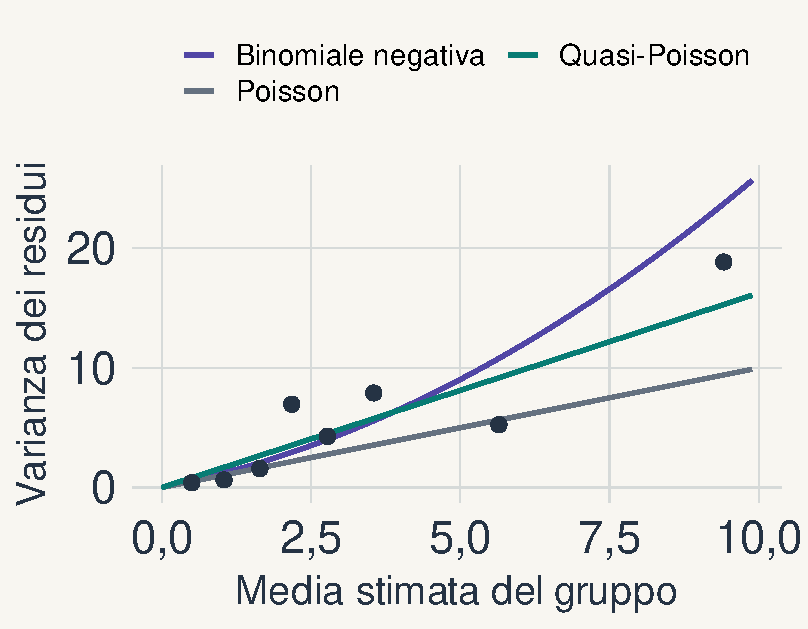
\includegraphics[width=\linewidth,height=6.15cm,keepaspectratio]{Figure/F04.pdf}\par}
\PSmall{Varianza dei residui in otto gruppi di celle ordinate per media stimata e tre funzioni di varianza.}
}};
\node[anchor=north west,inner sep=0] at([xshift=10.85cm,yshift=-2.12cm]current page.north west){\Colonna{8.16cm}{\PBody{Jay Ver Hoef e Peter Boveng confrontarono nel 2007 i due approcci: la varianza quasi-Poisson è lineare nella media, quella della binomiale negativa quadratica, e i pesi delle osservazioni cambiano di conseguenza. Nel caso i punti dei gruppi stanno fra le due curve; la binomiale negativa ha parametro di forma 6,19.}
\par\smallskip{\centering\adjustbox{max width=.98\linewidth}{$\displaystyle \operatorname{var}(Y)=\mu+\frac{\mu^2}{\theta}$}\par\smallskip}
}};
\end{tikzpicture}\end{frame}

\begin{frame}[plain]\hypertarget{slide19}{}
\bookmark[level=1,page=19]{La binomiale negativa per massima verosimiglianza}
\begin{tikzpicture}[remember picture,overlay]
\PilotChrome{La binomiale negativa per massima verosimiglianza}{SOVRADISPERSIONE}{19}{La binomiale negativa è un modello completo: stima anche il parametro di forma.}
\node[anchor=north west,inner sep=0] at([xshift=.96cm,yshift=-2.12cm]current page.north west){\Colonna{9.40cm}{\PBody{Il codice scrive la log-verosimiglianza con \texttt{dnbinom} e la massimizza con \texttt{optim}; l’inversa dell’hessiana fornisce gli errori standard. La pendenza vale 0,0918 con errore standard 0,0141 e il parametro di forma 6,19. \texttt{M20\_figure.R} verifica che il risultato coincide con \texttt{MASS::glm.nb}.}
\par\smallskip{\centering\adjustbox{max width=.98\linewidth}{$\displaystyle P(Y=y)=\frac{\Gamma(y+\theta)}{\Gamma(\theta)\,y!}\Big(\frac{\theta}{\theta+\mu}\Big)^{\theta}\Big(\frac{\mu}{\theta+\mu}\Big)^{y}$}\par\smallskip}
}};
\node[anchor=north west,inner sep=0] at([xshift=10.85cm,yshift=-2.12cm]current page.north west){\Colonna{8.16cm}{\begin{tcolorbox}[enhanced,arc=1.7mm,boxrule=.6pt,colback=white,colframe=Classical!60!Navy,colbacktitle=Navy,coltitle=white,fonttitle=\bfseries\small,title={R · calcolo riproducibile},left=1.7mm,right=1.3mm,top=1.1mm,bottom=1.1mm,before skip=1mm,after skip=1.0mm]\lstinputlisting[style=GeoR,language=R]{Codice/capitolo-06.R}\end{tcolorbox}
\PLabel{Risultato in R}
\begin{tcolorbox}[colback=GeoTint,colframe=Rule,boxrule=.5pt,arc=1.4mm,left=2mm,right=1mm,top=1mm,bottom=1mm]{\fontsize{8.6}{11.4}\selectfont\ttfamily \mbox{b\_pend\ \ \ \ \ se\ \ theta}\\\mbox{0.0918\ 0.0141\ 6.1933}}\end{tcolorbox}}};
\end{tikzpicture}\end{frame}

\begin{frame}[plain]\hypertarget{slide20}{}
\bookmark[level=1,page=20]{Tre intervalli per lo stesso effetto}
\begin{tikzpicture}[remember picture,overlay]
\PilotChrome{Tre intervalli per lo stesso effetto}{SOVRADISPERSIONE}{20}{Con sovradispersione l’intervallo di Poisson è troppo stretto.}
\node[anchor=north west,inner sep=0] at([xshift=.96cm,yshift=-2.12cm]current page.north west){\Colonna{9.40cm}{{\centering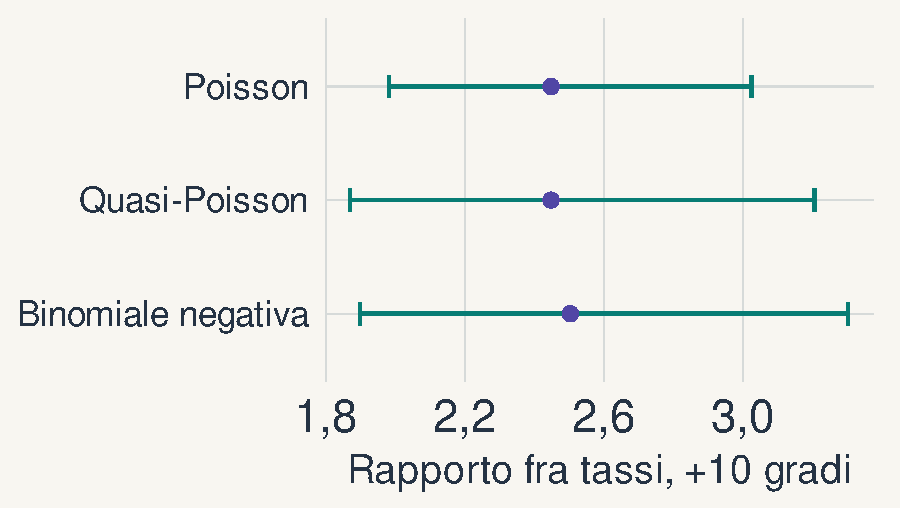
\includegraphics[width=\linewidth,height=6.15cm,keepaspectratio]{Figure/F05.pdf}\par}
\PSmall{Rapporto fra tassi per 10 gradi di pendenza con intervalli al 95\% dei tre modelli.}
}};
\node[anchor=north west,inner sep=0] at([xshift=10.85cm,yshift=-2.12cm]current page.north west){\Colonna{8.16cm}{\PBody{Le stime puntuali sono simili: 2,45 con Poisson e quasi-Poisson, 2,50 con la binomiale negativa. Gli intervalli si allargano: da 1,98–3,03 a 1,87–3,21 e 1,90–3,30. Il criterio di Akaike preferisce la binomiale negativa, 378,1 contro 387,1.}
\PSmall{Il criterio di Akaike non è definito per il modello quasi-Poisson, privo di una verosimiglianza.}
}};
\end{tikzpicture}\end{frame}

\begin{frame}[plain]\hypertarget{slide21}{}
\bookmark[level=1,page=21]{Da dove nasce la sovradispersione}
\begin{tikzpicture}[remember picture,overlay]
\PilotChrome{Da dove nasce la sovradispersione}{SOVRADISPERSIONE}{21}{La sovradispersione segnala variabilità non spiegata: va descritta e, se possibile, spiegata.}
\node[anchor=north west,inner sep=0] at([xshift=.96cm,yshift=-2.12cm]current page.north west){\Colonna{9.40cm}{\PLabel{Fattori non misurati}
\PBody{Il tasso di frane di una cella dipende anche da fattori assenti dal modello: piovosità, uso del suolo, fratturazione. Celle con la stessa pendenza e litologia hanno tassi diversi, e la loro miscela produce più zeri e più valori grandi di una Poisson. Nel generatore il fattore di cella segue una distribuzione gamma, che dà proprio una binomiale negativa.}
}};
\node[anchor=north west,inner sep=0] at([xshift=10.85cm,yshift=-2.12cm]current page.north west){\Colonna{8.16cm}{\PLabel{Che cosa scegliere}
\PBody{Quasi-Poisson e binomiale negativa hanno lo stesso numero di parametri. La scelta dipende da come la varianza cresce con la media nei dati, da controllare con un grafico come quello della tappa 18. Una sovradispersione può anche segnalare un predittore mancante o una forma sbagliata del predittore lineare.}
\PSmall{Dipendenza spaziale fra celle vicine produce effetti simili e richiede modelli spaziali.}
}};
\end{tikzpicture}\end{frame}

\begin{frame}[plain]\hypertarget{slide22}{}
\bookmark[level=1,page=22]{Sovradispersione e copertura degli intervalli}
\begin{tikzpicture}[remember picture,overlay]
\PilotChrome{Sovradispersione e copertura degli intervalli}{SOVRADISPERSIONE}{22}{Misurare la copertura degli intervalli di Poisson e quasi-Poisson con conteggi sovradispersi.}
\node[anchor=north west,inner sep=0] at([xshift=.96cm,yshift=-2.12cm]current page.north west){\Colonna{9.40cm}{{\centering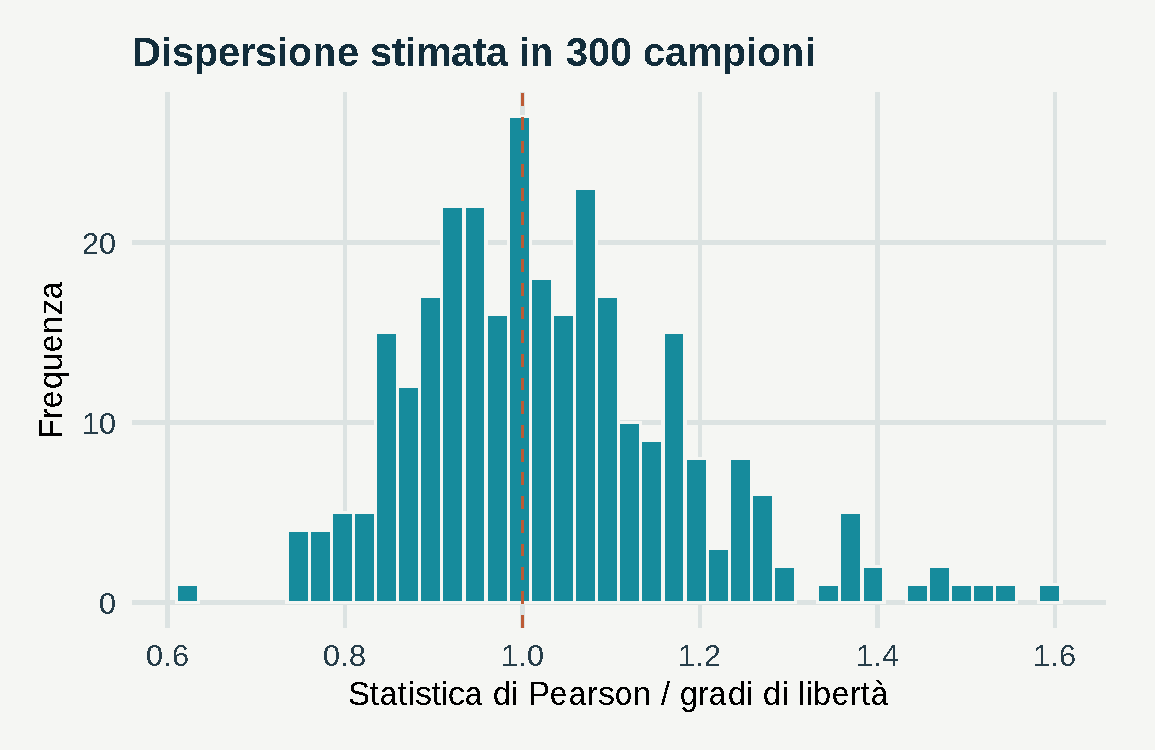
\includegraphics[width=\linewidth,height=6.0cm,keepaspectratio]{Esperimenti/m20-dispersione-A.pdf}\par}
\PSmall{Parametro di forma: 100; 96 celle; trecento campioni. Seme: 17.}
}};
\node[anchor=north west,inner sep=0] at([xshift=10.85cm,yshift=-2.12cm]current page.north west){\Colonna{8.16cm}{\PLabel{Scenario A · simulazione}
\PBody{L’esperimento genera conteggi da una binomiale negativa e adatta il modello di Poisson. Con $\theta=100$ la dispersione media è 1,03, e gli intervalli contengono la pendenza vera nel 93,7\% e nel 95,3\% dei campioni.}
\par\smallskip{\centering\adjustbox{max width=.98\linewidth}{$\displaystyle \hat\beta_1\pm1{,}96\,\mathrm{se}\sqrt{\max(1,\hat\phi)}$}\par\smallskip}
\PSmall{Con media 3 la varianza della binomiale negativa è $3+9/\theta$.}
}};
\node[anchor=north east,inner sep=0] at([xshift=17.1cm,yshift=-12.04cm]current page.north west){\fontsize{7.7}{9}\selectfont \href{https://marzione00.github.io/Lab_Geo/\#laboratorio/m20-dispersione}{\color{Classical}\bfseries Apri il laboratorio · m20-dispersione}};
\end{tikzpicture}\end{frame}

\begin{frame}[plain]\hypertarget{slide23}{}
\bookmark[level=1,page=23]{Confronto | Sovradispersione e copertura}
\begin{tikzpicture}[remember picture,overlay]
\PilotChrome{Confronto | Sovradispersione e copertura}{SOVRADISPERSIONE}{23}{Correggere gli errori standard per la dispersione riporta la copertura vicino al valore nominale.}
\node[anchor=north west,inner sep=0] at([xshift=.96cm,yshift=-2.12cm]current page.north west){\Colonna{9.40cm}{{\centering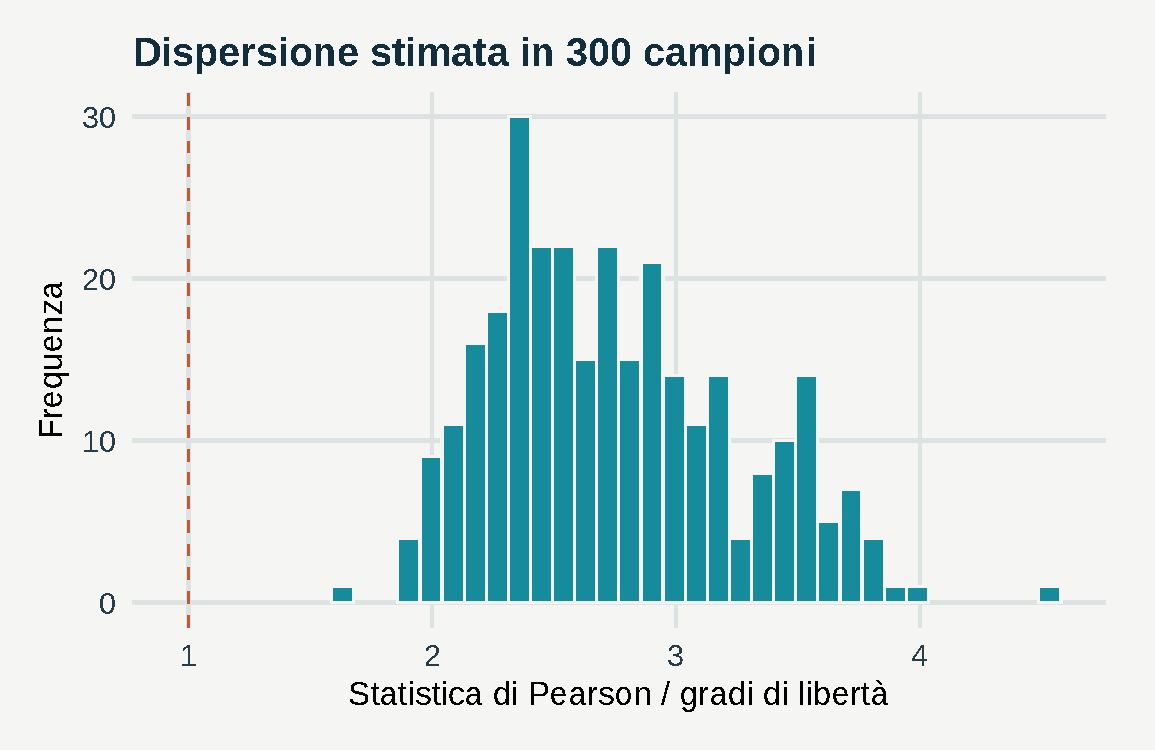
\includegraphics[width=\linewidth,height=5.6cm,keepaspectratio]{Esperimenti/m20-dispersione-B.pdf}\par}
\PSmall{Parametro di forma: 100 $\to$ 2. Tutti gli altri parametri e il seme sono fissi.}
}};
\node[anchor=north west,inner sep=0] at([xshift=10.85cm,yshift=-2.12cm]current page.north west){\Colonna{8.16cm}{\PLabel{Confronto fra gli scenari}
{\fontsize{10.2}{12.8}\selectfont\begin{tabular}{@{}>{\raggedright\arraybackslash}p{0.48\linewidth}@{\hspace{.13cm}}>{\raggedright\arraybackslash}p{0.224\linewidth}@{\hspace{.13cm}}>{\raggedright\arraybackslash}p{0.224\linewidth}@{}}\toprule Grandezza & A & B\\[2.3pt]
\midrule 
Dispersione media & 1{,}03 & 2{,}75\\[2.3pt]
Varianza attesa a media 3 & 3{,}09 & 7{,}5\\[2.3pt]
Copertura, Poisson & 0{,}937 & 0{,}757\\[2.3pt]
Copertura, quasi-Poisson & 0{,}953 & 0{,}933\\[2.3pt]
\bottomrule\end{tabular}\par}
\vspace{.25cm}\PBody{Con $\theta=2$ la dispersione media sale a 2,75 e l’intervallo di Poisson contiene la pendenza vera soltanto nel 75,7\% dei campioni; quello quasi-Poisson nel 93,3\%.}
}};
\node[anchor=north east,inner sep=0] at([xshift=17.1cm,yshift=-12.04cm]current page.north west){\fontsize{7.7}{9}\selectfont \href{https://marzione00.github.io/Lab_Geo/\#laboratorio/m20-dispersione}{\color{Classical}\bfseries Apri il laboratorio · m20-dispersione}};
\end{tikzpicture}\end{frame}

\begin{frame}[plain]\hypertarget{slide24}{}
\bookmark[level=0,page=24]{Proporzioni e regressione logistica}
\bookmark[level=1,page=24]{Una retta per le proporzioni?}
\begin{tikzpicture}[remember picture,overlay]
\PilotChrome{Una retta per le proporzioni?}{PROPORZIONI E REGRESSIONE LOGISTICA}{24}{Una proporzione sta fra 0 e 1; una retta no.}
\node[anchor=north west,inner sep=0] at([xshift=.96cm,yshift=-2.12cm]current page.north west){\Colonna{9.40cm}{\PLabel{Domanda}
\PBody{Il feldspato diminuisce lungo il percorso di trasporto. Che cosa prevede una retta adattata alle frazioni misurate per una stazione a 90 km, oltre l’ultima stazione campionata?}
\vspace{.35cm}\PLabel{Interpretazione}
\PBody{La retta prevede 0,309 all’origine, 0,040 a 60 km e $-0{,}095$ a 90 km: una frazione negativa. Anche dentro l’intervallo la retta ignora che la variabilità di una frazione dipende dal suo valore.}
}};
\node[anchor=north west,inner sep=0] at([xshift=10.85cm,yshift=-2.12cm]current page.north west){\Colonna{8.16cm}{\begin{tcolorbox}[enhanced,arc=1.7mm,boxrule=.6pt,colback=white,colframe=Classical!60!Navy,colbacktitle=Navy,coltitle=white,fonttitle=\bfseries\small,title={R · calcolo riproducibile},left=1.7mm,right=1.3mm,top=1.1mm,bottom=1.1mm,before skip=1mm,after skip=1.0mm]\lstinputlisting[style=GeoR,language=R]{Codice/capitolo-07.R}\end{tcolorbox}
\PLabel{Risultato in R}
\begin{tcolorbox}[colback=GeoTint,colframe=Rule,boxrule=.5pt,arc=1.4mm,left=2mm,right=1mm,top=1mm,bottom=1mm]{\fontsize{8.6}{11.4}\selectfont\ttfamily \mbox{\ \ \ \ \ 1\ \ \ \ \ \ 2\ \ \ \ \ \ 3}\\\mbox{\ 0.309\ \ 0.040\ -0.095}}\end{tcolorbox}}};
\end{tikzpicture}\end{frame}

\begin{frame}[plain]\hypertarget{slide25}{}
\bookmark[level=1,page=25]{Il feldspato lungo il trasporto}
\begin{tikzpicture}[remember picture,overlay]
\PilotChrome{Il feldspato lungo il trasporto}{PROPORZIONI E REGRESSIONE LOGISTICA}{25}{La curva logistica si avvicina a zero senza attraversarlo.}
\node[anchor=north west,inner sep=0] at([xshift=.96cm,yshift=-2.12cm]current page.north west){\Colonna{9.40cm}{{\centering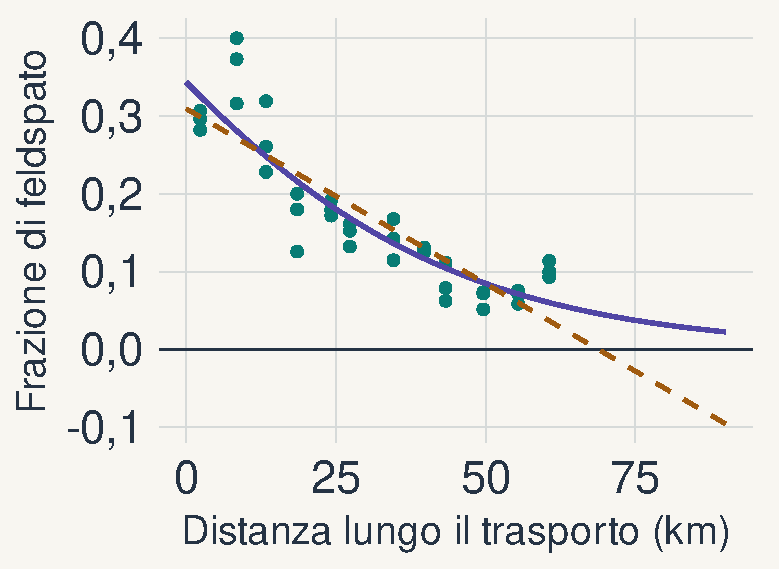
\includegraphics[width=\linewidth,height=6.15cm,keepaspectratio]{Figure/F06.pdf}\par}
\PSmall{Frazione di feldspato nelle 36 sezioni; curva: modello logistico; tratteggio: retta dei minimi quadrati.}
}};
\node[anchor=north west,inner sep=0] at([xshift=10.85cm,yshift=-2.12cm]current page.north west){\Colonna{8.16cm}{\PBody{Il modello logistico stima una frazione di 0,343 all’origine, 0,061 a 60 km e 0,023 a 90 km. David Cox pubblicò nel 1958 la regressione per risposte binarie con il legame logistico, la forma usata qui per conteggi di successi su un numero noto di prove.}
\par\smallskip{\centering\adjustbox{max width=.98\linewidth}{$\displaystyle \log\frac{p_i}{1-p_i}=\beta_0+\beta_1d_i$}\par\smallskip}
\PSmall{$K_i\sim\mathrm{Bin}(n_i,p_i)$: punti di feldspato $K_i$ su $n_i$ punti contati alla distanza $d_i$.}
}};
\end{tikzpicture}\end{frame}

\begin{frame}[plain]\hypertarget{slide26}{}
\bookmark[level=1,page=26]{Il modello binomiale e la sua dispersione}
\begin{tikzpicture}[remember picture,overlay]
\PilotChrome{Il modello binomiale e la sua dispersione}{PROPORZIONI E REGRESSIONE LOGISTICA}{26}{Le sezioni di una stessa roccia differiscono più di quanto il solo conteggio preveda.}
\node[anchor=north west,inner sep=0] at([xshift=.96cm,yshift=-2.12cm]current page.north west){\Colonna{9.40cm}{\PBody{Il coefficiente della distanza vale $-0{,}0346$ per km: ogni 10 km le probabilità a favore del feldspato si moltiplicano per 0,707. La dispersione vale 3,56, e l’errore standard quasi-binomiale passa da 0,0016 a 0,0029. Le sezioni hanno una variabilità oltre quella del conteggio.}
\par\smallskip{\centering\adjustbox{max width=.98\linewidth}{$\displaystyle \frac{p/(1-p)\,\big|_{d+10}}{p/(1-p)\,\big|_{d}}=e^{10\beta_1}$}\par\smallskip}
}};
\node[anchor=north west,inner sep=0] at([xshift=10.85cm,yshift=-2.12cm]current page.north west){\Colonna{8.16cm}{\begin{tcolorbox}[enhanced,arc=1.7mm,boxrule=.6pt,colback=white,colframe=Classical!60!Navy,colbacktitle=Navy,coltitle=white,fonttitle=\bfseries\small,title={R · calcolo riproducibile},left=1.7mm,right=1.3mm,top=1.1mm,bottom=1.1mm,before skip=1mm,after skip=1.0mm]\lstinputlisting[style=GeoR,language=R]{Codice/capitolo-08.R}\end{tcolorbox}
\PLabel{Risultato in R}
\begin{tcolorbox}[colback=GeoTint,colframe=Rule,boxrule=.5pt,arc=1.4mm,left=2mm,right=1mm,top=1mm,bottom=1mm]{\fontsize{8.6}{11.4}\selectfont\ttfamily \mbox{\ \ \ \ \ \ \ b\ \ \ \ \ \ \ se\ \ \ \ \ \ phi\ se\_quasi\ \ OR\_10km}\\\mbox{\ -0.0346\ \ \ 0.0016\ \ \ 3.5628\ \ \ 0.0029\ \ \ 0.7074}}\end{tcolorbox}}};
\end{tikzpicture}\end{frame}

\begin{frame}[plain]\hypertarget{slide27}{}
\bookmark[level=1,page=27]{Errore di conteggio ed errore di campione}
\begin{tikzpicture}[remember picture,overlay]
\PilotChrome{Errore di conteggio ed errore di campione}{PROPORZIONI E REGRESSIONE LOGISTICA}{27}{L’errore binomiale del conteggio è soltanto una parte dell’incertezza di una frazione.}
\node[anchor=north west,inner sep=0] at([xshift=.96cm,yshift=-2.12cm]current page.north west){\Colonna{9.40cm}{\PLabel{Errore di conteggio}
\PBody{L. van der Plas e A. C. Tobi pubblicarono nel 1965 un diagramma per giudicare l’affidabilità del conteggio per punti, basato su due deviazioni standard binomiali; la distanza fra i punti deve superare la dimensione del granulo più grande. Con 300 punti e una frazione del 25\% la deviazione standard è 0,025.}
\par\smallskip{\centering\adjustbox{max width=.98\linewidth}{$\displaystyle \sigma_p=\sqrt{\frac{p(1-p)}{n}}$}\par\smallskip}
}};
\node[anchor=north west,inner sep=0] at([xshift=10.85cm,yshift=-2.12cm]current page.north west){\Colonna{8.16cm}{\PLabel{Errore di campione}
\PBody{F. Chayes scompose nel 1956 l’errore di un’analisi modale in errore di conteggio ed errore di campione. M. J. Neilson e G. F. Brockman raccomandarono nel 1977 di contare i punti in più serie e di stimare l’errore dalla deviazione standard campionaria. Nel caso la varianza fra le tre sezioni di una stazione è 1,46 volte quella binomiale.}
\PSmall{Nel generatore ogni stazione ha un effetto casuale sulla scala logit e ogni sezione un piccolo scarto proprio.}
}};
\end{tikzpicture}\end{frame}

\begin{frame}[plain]\hypertarget{slide28}{}
\bookmark[level=1,page=28]{Probabilità, probabilità a favore e logit}
\begin{tikzpicture}[remember picture,overlay]
\PilotChrome{Probabilità, probabilità a favore e logit}{PROPORZIONI E REGRESSIONE LOGISTICA}{28}{Un coefficiente logistico moltiplica le probabilità a favore, $p/(1-p)$.}
\node[anchor=north west,inner sep=0] at([xshift=.96cm,yshift=-2.12cm]current page.north west){\Colonna{9.40cm}{{\centering\resizebox{0.94\linewidth}{!}{\begin{tikzpicture}[x=1cm,y=1cm,every node/.append style={anchor=center,inner sep=.3333em}]
\draw[-{Latex[length=2mm]},Ink,line width=.6pt] (-3.4,0)--(3.6,0) node[pNote,anchor=north east]{$\eta=\log\frac{p}{1-p}$};
\draw[-{Latex[length=2mm]},Ink,line width=.6pt] (0,-.2)--(0,3.1) node[pNote,anchor=south]{$p$};
\draw[Muted,dashed] (-3.3,2.6)--(3.3,2.6);
\node[pNote,anchor=east] at(-.05,2.6){1};
\draw[GeoA,line width=1.4pt,domain=-3.3:3.3,samples=80] plot(\x,{2.6/(1+exp(-1.3*\x))});
\fill[GeoB] (0,1.3) circle(2.2pt) node[pLabel,anchor=west,text=GeoB]{\ $p=0{,}5$};
\node[pNote,text width=7.3cm] at(0,-1.25){Il logit porta l’intervallo $(0,1)$ sull’intera retta. Un coefficiente $\beta$ moltiplica le probabilità a favore, $p/(1-p)$, per $e^{\beta}$ a ogni unità del predittore.};
\end{tikzpicture}
}\par}
\PSmall{Curva logistica fra il predittore lineare e la probabilità.}
}};
\node[anchor=north west,inner sep=0] at([xshift=10.85cm,yshift=-2.12cm]current page.north west){\Colonna{8.16cm}{\PBody{Il legame logistico porta una probabilità fra 0 e 1 sull’intera retta reale. Una variazione unitaria del predittore moltiplica le probabilità a favore per $e^{\beta}$; l’effetto sulla probabilità dipende dal punto della curva, massimo attorno a 0,5 e piccolo vicino a 0 e a 1.}
\par\smallskip{\centering\adjustbox{max width=.98\linewidth}{$\displaystyle p=\frac{1}{1+e^{-\eta}},\qquad \frac{dp}{d\eta}=p(1-p)$}\par\smallskip}
}};
\end{tikzpicture}\end{frame}

\begin{frame}[plain]\hypertarget{slide29}{}
\bookmark[level=1,page=29]{Punti contati e variabilità fra stazioni}
\begin{tikzpicture}[remember picture,overlay]
\PilotChrome{Punti contati e variabilità fra stazioni}{PROPORZIONI E REGRESSIONE LOGISTICA}{29}{Valutare quanto contare più punti per sezione migliora la stima quando le stazioni differiscono.}
\node[anchor=north west,inner sep=0] at([xshift=.96cm,yshift=-2.12cm]current page.north west){\Colonna{9.40cm}{{\centering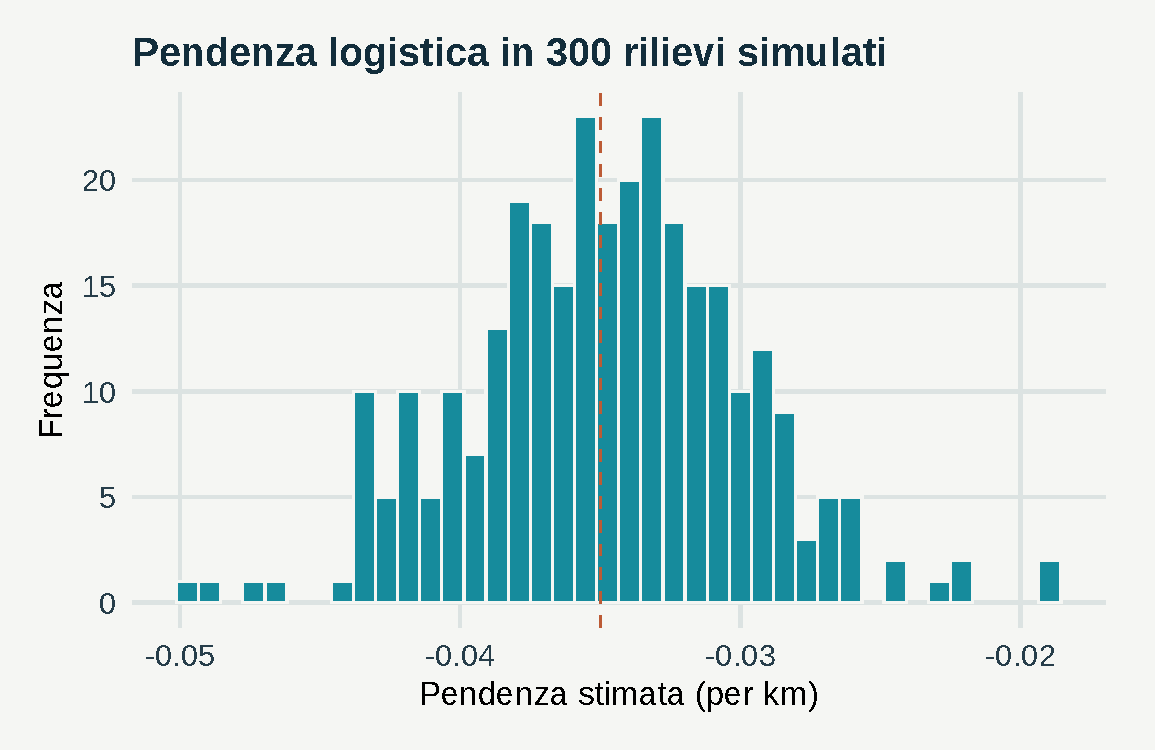
\includegraphics[width=\linewidth,height=6.0cm,keepaspectratio]{Esperimenti/m20-punti-A.pdf}\par}
\PSmall{Cento punti per sezione; variabilità fra stazioni 0,25 sulla scala logit. Seme: 17.}
}};
\node[anchor=north west,inner sep=0] at([xshift=10.85cm,yshift=-2.12cm]current page.north west){\Colonna{8.16cm}{\PLabel{Scenario A · simulazione}
\PBody{L’esperimento simula trecento rilievi di dodici stazioni con tre sezioni ciascuna. Con cento punti per sezione la deviazione standard delle pendenze è 0,00485, l’errore standard binomiale medio 0,00265 e quello quasi-binomiale 0,00346.}
\par\smallskip{\centering\adjustbox{max width=.98\linewidth}{$\displaystyle \operatorname{logit}p_{ij}=\beta_0+\beta_1d_j+u_j$}\par\smallskip}
\PSmall{$u_j$ è l’effetto della stazione $j$, comune alle sue tre sezioni.}
}};
\node[anchor=north east,inner sep=0] at([xshift=17.1cm,yshift=-12.04cm]current page.north west){\fontsize{7.7}{9}\selectfont \href{https://marzione00.github.io/Lab_Geo/\#laboratorio/m20-punti}{\color{Classical}\bfseries Apri il laboratorio · m20-punti}};
\end{tikzpicture}\end{frame}

\begin{frame}[plain]\hypertarget{slide30}{}
\bookmark[level=1,page=30]{Confronto | Punti contati e variabilità fra stazioni}
\begin{tikzpicture}[remember picture,overlay]
\PilotChrome{Confronto | Punti contati e variabilità fra stazioni}{PROPORZIONI E REGRESSIONE LOGISTICA}{30}{Oltre un certo numero di punti l’incertezza dipende dal numero di stazioni.}
\node[anchor=north west,inner sep=0] at([xshift=.96cm,yshift=-2.12cm]current page.north west){\Colonna{9.40cm}{{\centering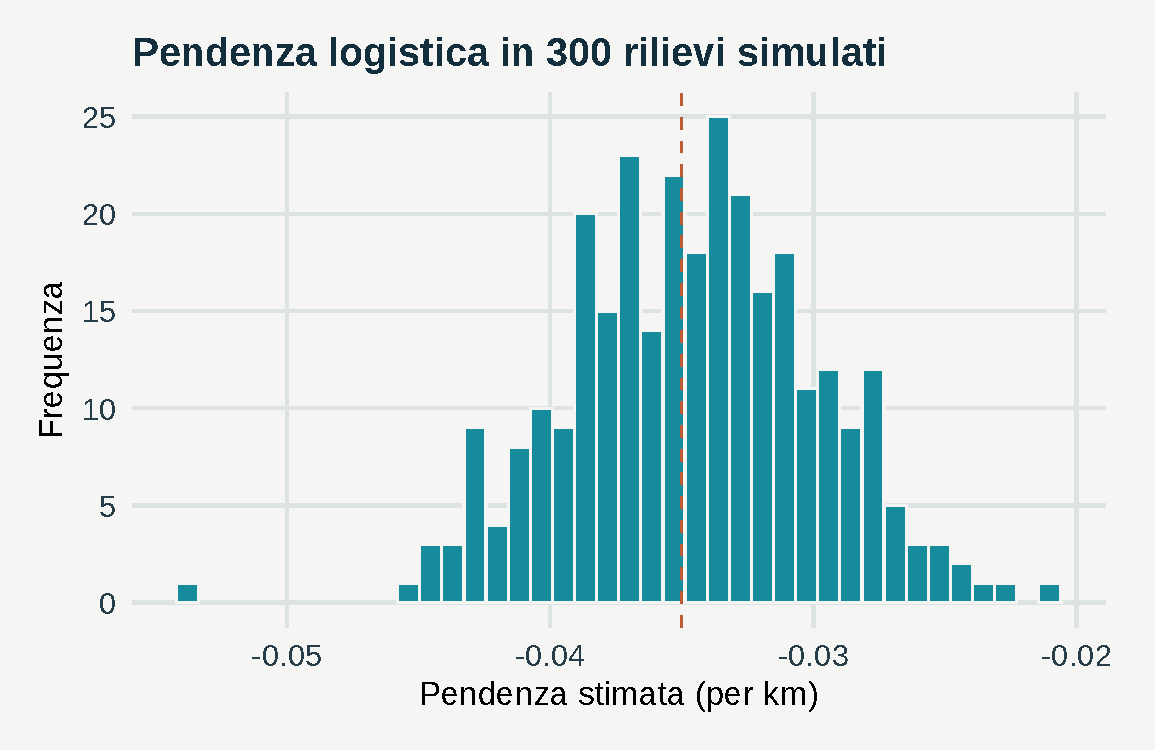
\includegraphics[width=\linewidth,height=5.6cm,keepaspectratio]{Esperimenti/m20-punti-B.pdf}\par}
\PSmall{Punti per sezione: 100 $\to$ 1000. Tutti gli altri parametri e il seme sono fissi.}
}};
\node[anchor=north west,inner sep=0] at([xshift=10.85cm,yshift=-2.12cm]current page.north west){\Colonna{8.16cm}{\PLabel{Confronto fra gli scenari}
{\fontsize{10.2}{12.8}\selectfont\begin{tabular}{@{}>{\raggedright\arraybackslash}p{0.48\linewidth}@{\hspace{.13cm}}>{\raggedright\arraybackslash}p{0.224\linewidth}@{\hspace{.13cm}}>{\raggedright\arraybackslash}p{0.224\linewidth}@{}}\toprule Grandezza & A & B\\[2.3pt]
\midrule 
Dev. standard delle pendenze & 0{,}00485 & 0{,}00472\\[2.3pt]
Errore standard binomiale & 0{,}00265 & 0{,}000837\\[2.3pt]
Errore standard quasi-binomiale & 0{,}00346 & 0{,}00237\\[2.3pt]
Dispersione media & 1{,}74 & 8{,}48\\[2.3pt]
\bottomrule\end{tabular}\par}
\vspace{.25cm}\PBody{Con mille punti l’incertezza reale resta 0,00472: l’errore binomiale scende a 0,00084 e quello quasi-binomiale a 0,00237. Le sezioni di una stazione condividono lo stesso effetto e le loro frazioni sono correlate.}
}};
\node[anchor=north east,inner sep=0] at([xshift=17.1cm,yshift=-12.04cm]current page.north west){\fontsize{7.7}{9}\selectfont \href{https://marzione00.github.io/Lab_Geo/\#laboratorio/m20-punti}{\color{Classical}\bfseries Apri il laboratorio · m20-punti}};
\end{tikzpicture}\end{frame}

\begin{frame}[plain]\hypertarget{slide31}{}
\bookmark[level=0,page=31]{Sintesi}
\bookmark[level=1,page=31]{Dal risultato alla relazione}
\begin{tikzpicture}[remember picture,overlay]
\PilotChrome{Dal risultato alla relazione}{SINTESI}{31}{Riporta distribuzione, legame, offset, dispersione e intervalli dei rapporti stimati.}
\node[anchor=north west,inner sep=0] at([xshift=.96cm,yshift=-2.12cm]current page.north west){\Colonna{9.40cm}{\PLabel{Domanda di partenza}
\PBody{Quanto aumenta il tasso di frane con la pendenza?}
\PLabel{Risultato da discutere}
\PBody{Dieci gradi di pendenza moltiplicano il tasso di frane per circa 2,5, con intervallo da 1,9 a 3,3 se si tiene conto della sovradispersione; flysch e calcari hanno tassi pari a circa metà e un quarto di quello delle argille. Lungo il trasporto le probabilità a favore del feldspato si riducono del 29\% ogni 10 km.}
}};
\node[anchor=north west,inner sep=0] at([xshift=10.85cm,yshift=-2.12cm]current page.north west){\Colonna{8.16cm}{\PLabel{Limiti della conclusione}
\PBody{I dati sono sintetici e le celle indipendenti. La sovradispersione è trattata con modelli che non spiegano la sua origine, e il conteggio per punti ha una struttura per stazioni che un modello a effetti casuali descriverebbe meglio.}
\vspace{.4cm}\href{https://marzione00.github.io/Lab_Geo/\#modulo-M20}{\color{Classical}\bfseries Torna agli esperimenti di Numerus}
}};
\end{tikzpicture}\end{frame}

\begin{frame}[plain]\hypertarget{slide32}{}
\bookmark[level=0,page=32]{Riferimenti}
\bookmark[level=1,page=32]{Fonti, dati e codice per riprodurre le figure}
\begin{tikzpicture}[remember picture,overlay]
\PilotChrome{Fonti, dati e codice per riprodurre le figure}{RIFERIMENTI}{32}{I risultati numerici si riferiscono ai dati e alle ipotesi dichiarate nel caso.}
\node[anchor=north west,inner sep=0] at([xshift=.96cm,yshift=-2.12cm]current page.north west){\Colonna{9.40cm}{\PLabel{Fonti}
{\fontsize{9.4}{12.2}\selectfont S. D. Poisson, Recherches sur la probabilité des jugements, Bachelier, 1837.\par F. Chayes, Petrographic Modal Analysis, Wiley, 1956.\par D. R. Cox, Journal of the Royal Statistical Society B 20(2), 215–242, 1958.\par L. van der Plas e A. C. Tobi, American Journal of Science 263(1), 87–90, 1965.\par J. A. Nelder e R. W. M. Wedderburn, Journal of the Royal Statistical Society A 135(3), 370–384, 1972.\par R. W. M. Wedderburn, Biometrika 61(3), 439–447, 1974.\par M. J. Neilson e G. F. Brockman, American Mineralogist 62, 1238–1244, 1977.\par P. McCullagh e J. A. Nelder, Generalized Linear Models, 2ª ed., Chapman and Hall, 1989.\par J. M. Ver Hoef e P. L. Boveng, Ecology 88(11), 2766–2772, 2007.\par}
}};
\node[anchor=north west,inner sep=0] at([xshift=10.85cm,yshift=-2.12cm]current page.north west){\Colonna{8.16cm}{\PLabel{Dati e codice}
\PBody{Dati sintetici del corso (frane\_v1.csv, conteggi\_v1.csv), generati da R/genera\_dati.R. Codice contiene i frammenti delle pagine; R/M20\_figure.R ricostruisce figure e valori; Esperimenti contiene i programmi dei due scenari e Diagrammi i disegni TikZ.}
\vspace{.3cm}\href{https://marzione00.github.io/Lab_Geo/\#lezione-M20}{\color{Classical}\bfseries Apri le tappe di Numerus su GeoStat Lab}
}};
\end{tikzpicture}\end{frame}
\end{document}
